\documentclass[a4paper, titlepage]{article}
\usepackage{HYY_style}
\usepackage{setspace, changepage, enumitem, verbatim}
\usepackage{tikz}
\usepackage[utf8]{inputenc}
\usepackage[T1]{fontenc}
\usepackage{lmodern}
\usepackage{epstopdf}
\usepackage{matlab}
\usepackage{enumitem}
\usepackage{longtable, booktabs, multirow, makecell, threeparttable, ltxtable, supertabular, array, float}
\newcommand{\tabincell}[2]{\begin{tabular}{@{}#1@{}}#2\end{tabular}}
\allowdisplaybreaks[4]
\geometry{top=25mm,bottom=25mm,left=30mm,right=30mm}
\begin{document}
    \renewcommand{\thefootnote}{\fnsymbol{footnote}}
    \title{{\small《MATLAB程序设计》大作业个人汇报}\\COVID-19疫情数据的简要统计分析与预测\footnotemark[1]}
    \author{王逸扬(19300180016)\\杨耕智(19300180112){\kaishu }}
    \date{2022年5月21日}
    \footnotetext[1]{\kaishu 相关代码及其版本演进托管在\url{https://github.com/maix00/StatisticsAnalysis}.}
    \maketitle
    \renewcommand{\thefootnote}{\araboc{footnote}}
    \thispagestyle{empty}
    \renewcommand{\contentsname}{\centering 目录\\\quad\\}
    \tableofcontents
    \thispagestyle{empty}
    \newpage
    \pagestyle{headings}
   

    \section{整体分析思路}
          众所周知,2019年底开始的COVID-19疫情给人们的生产生活造成了极大的影响,如何利用疫情相关数据、如何通过数据挖掘、分析、预测,以指导人们作出更加有利于社会发展的决策,是当今较为热门的研究方向. 在此,我们将根据所给的有关数据,尽可能地贴合这个目的,做出一些简要的分析与预测.

        \subsection{数据观察与简要分析}
          首先,观察所给数据. 有两个数据集,一个是\texttt{country.csv}(以下称「地区数据」),另一个是\texttt{daily\_info.csv}(以下称「每日数据」). 
        \subsubsection*{地区数据}
          地区数据中共有$229$条数据,每个地区最多有$12$个特征,简要分类:
        \vspace{5pt}
        \begin{adjustwidth}{1cm}{0cm}
        {\kaishu
        \begin{itemize}[itemsep=-1pt]
            \item [\textbf{地理位置}:]
                所属大洲               \texttt{continent}
            \item [\textbf{人口成分}:]
                人口                 \texttt{population}\\ 
                每平方千米人口密度          \texttt{population\_density}; \\
                中位年龄               \texttt{median\_age}\\
                $65$岁以上人口占比          \hspace{1.1em}\texttt{aged\_65\_older}\\
                $70$岁以上人口占比          \hspace{1.1em}\texttt{aged\_70\_older}
            \item [\textbf{经济环境}:]
                按购买力平价的人均国民生产总值    \texttt{gdp\_per\_capita}
            \item [\textbf{卫生水平}:]
                男性吸烟率              \texttt{male\_smokers}\\ 
                女性吸烟率              \texttt{female\_smokers}\\ 
                每年每十万人心血管疾病死亡率     \texttt{cardiovasc\_death\_rate}\\ 
                每千人床位数             \texttt{hospital\_beds\_per\_thousands}\\ 
                预期寿命               \texttt{life\_expectancy}
        \end{itemize}
        }
        \end{adjustwidth}
        \vspace{5pt}
        根据这些特征数据,我们可以对这些地区进行无监督聚类分析,但需要事先对缺失值进行处理(见节\ref{数据的缺失值处理}). 此后,我们可以在每一类中选取一个代表性的地区构建一分析预测模型(利用每日数据和/或地区特征),并可对同一类中的其他地区验证该模型的有效性. 这是本文开展分析的\textbf{第一种路径}.
        
          但是,需要预先指出如下两点:
        \begin{enumerate}[itemsep=-2pt,topsep=1pt]
            \item [(1)] 因为所给数据的有限性,所能建立或选择的模型是有限的,这里的特征作为模型参数的个数也是有限的,因此这里的多数特征在本文中只能用于聚类.
            \item [(2)] 某个地区其疫情的发展特征,可能与这里列明的某个特征相关性较低,此时,如果这个特征对上述的聚类分析产生过较大的影响,那么最终所获得分析预测模型,可能将不适用于该国所在类的其他地区.
        \end{enumerate}
        我们将在随后的数据分析中考虑这些问题,酌情选取模型.

        \subsubsection*{每日数据}
          对于每日数据,我们首先指出,对于其数据导入与缺失值处理上遇到的问题,我们将在节\ref{数据的导入}与节\ref{数据的缺失值处理}中分别尝试解决. 下面,对每日数据的各字段(除所属大洲与时间戳外),简要分类:
        \vspace{5pt}
        \begin{adjustwidth}{1cm}{0cm}
        {\kaishu
        \begin{itemize}[itemsep=-1pt,topsep=1pt]
            \item [\textbf{严重程度}:] 
                新增与累计病例        \texttt{new\_cases}, \texttt{total\_cases}\\
                住院与重症监护ICU人数   \hspace{1em}\texttt{hosp\_patients}, \texttt{icu\_patients}\\
                近七日平均检测阳性率     \texttt{positive\_rate}
            \item [\textbf{检测能力}:]
                新增与累计检测人次      \texttt{new\_tests}, \texttt{total\_tests}\\
                近七日平均检测阳性率     \texttt{positive\_rate}
            \item [\textbf{疫苗接种}:] 
                新增与累计疫苗接种人次    \texttt{new\_vaccinations}, \texttt{total\_vaccinations}
            \item [\textbf{管控力度}:] 
                政府管控力度         \texttt{stringency\_index}
        \end{itemize}
        }
        \end{adjustwidth}
        \vspace{5pt}
        这些时间序列数据,(1)可以用来构建一分析预测模型,(2)也可以取某一时间段内的最大、平均等统计指标(时间序列特征),用来对不同地区进行无监督聚类分析. 这里的聚类分析,得到的是不同地区的不同疫情发展模式,与前面的利用地区数据得到的关于地区特性的聚类不同. 针对不同的发展模式,可以提出更有针对性的建议,这是本文开展分析的\textbf{第二种路径}.

          另外,需要预先指出,因为所给数据的有限性,所能建立或选择的分析预测模型是极其有限的,比如,由于缺少治愈、死亡数据,不能采用传统的传染病模型SIR至SEIR等,又比如,由于缺少流调数据,无法统计计算基本再生数$R_0$、潜伏期平均长度$\bar{T_L}$等与传染病有关的统计指标. 

        \subsection{整体分析思路}
          综合上面的简要分析,我们将本文的整体分析思路概括如下. 首先,我们将利用自回归与偏自回归分析,对疫情的长期发展趋势给出一个简要说明. 其次,我们将遵循以下两种不同的路径对疫情的短期性特征展开分析.

        \paragraph{\fbox{第一种路径}} \textbf{基于LSTM神经网络模型的预测分析}
        \vspace{5pt}
        \begin{adjustwidth}{1cm}{0cm}
        {\kaishu
        \begin{itemize}[itemsep=-1pt,topsep=1pt]
            \item [\textbf{第一步}:](聚类分析)利用聚类方法,对地区数据进行缺失值处理,并进一步开展聚类分析.
            \item [\textbf{第二步}:](构建模型)对每日数据,基于LSTM神经网络模型,对代表地区一定时期内的每日病例数据进行学习.
            \item [\textbf{第三步}:](预测检验)利用上一步得到的模型,对时期外的数据进行预测检验,并对同一类中的其他地区的数据进行预测检验.
        \end{itemize}
        }
        \end{adjustwidth}
        \vspace{5pt}
        
        \paragraph{\fbox{第二种路径}} \textbf{基于时间序列特征的谱系聚类}
        \vspace{5pt}
        \begin{adjustwidth}{1cm}{0cm}
        {\kaishu
        \begin{itemize}[itemsep=-1pt,topsep=1pt]
            \item [\textbf{第一步}:](构造特征)划定区间,对每日数据进行缺失值处理,并进一步获取时间序列特征.
            \item [\textbf{第二步}:](聚类分析)根据以上时间序列特征,进行谱系聚类.
            \item [\textbf{第三步}:](政策建议)对具有不同疫情发展特征的地区,尝试作出政策建议.
        \end{itemize}
        }
        \end{adjustwidth}
        %\url{https://www.it610.com/article/1515470890224123904.html}.

        \subsection{说明}
          因为疫情的关系,我们两位同学,不得不线上联系,我们也因此第一次尝试使用github平台. 仓库网址为\url{https://github.com/maix00/StatisticsAnalysis}. 在那里,我们利用MATLAB的面向对象编程,编写了一个类\texttt{StatisticsAnalysis},用于辅助导入数据、检索表格、缺失值处理等,这在本文中会被用到,用到时我们会详细说明.

          本文的第\ref{数据的导入}节、第\ref{数据的缺失值处理}节将分别涉及数据的导入与缺失值处理中遇到的问题;第\ref{自相关分析}节进行自相关分析;第节、第节分别涉及上述两种不同路径的分析;第\ref{可视化}探索其他可能的数据可视化与数据分析.
        
          附录部分,附录\ref{app:StatisticsAnalysis}给出关于类\texttt{StatisticsAnalysis}的详细说明,附录\ref{存储结构}给出本文所依赖的MATLAB代码的存储方式.

          祝阅读愉快!
    
    \newpage
    \section{数据的导入与检索}\label{数据的导入}
        导入数据已有可以使用的\texttt{readtable}函数,且可以通过\texttt{detectImportOptions}函数,在导入数据前,预先探测并修改导入参数. 在此过程中,我们发现如下问题:
        \begin{enumerate}
            \item [1.] 以每日数据的\texttt{new\_vaccinations}与\texttt{total\_vaccinations}变量为例. 由于疫情发生初期长时间没有此类数据,\texttt{detectImportOptions}函数探测认为,此变量的变量类型是为\texttt{char},因此需要手动将导入参数修改为\texttt{double}.
            \item [2.] 在导入每日数据时,通常最后需要检索出某个地区、某个时间段的数据,目的是形成时序数据. 为此,MATLAB可以通过括号索引检索,但是不同类型的数据检索的方式不同,不是很便利,没有专门的检索函数可以使用.
        \end{enumerate}
        为了解决上面发现的问题,并寄希望于能在单一函数中解决全部的导入与检索问题,我们利用MATLAB面向对象变成,编写了类\texttt{StatisticsAnalysis}. {\color{red}
        \kaishu 注意:使用时请添加路径,或者在MATLAB中打开\texttt{./Project.prj}以自动添加路径.} 比如,我们想要导入法国在2020年的新增与累计接种疫苗人次——
\begin{matlabcode}
daily_SA = StatisticsAnalysis( ...
    'TablePath', './data/COVID19/daily_info.csv', ...
    'ImportOptions', { ...
        'VariableTypes', { ...
            'new_vaccinations', 'double', ...
            'total_vaccinations', 'double' ...
            }, ...
        'SelectedVariableNames', ...
            {'date', 'new_vaccinations', 'total_vaccinations'} ...
        }, ...
    'SelectTableOptions', { ...
        'location', 'France', ...
        'date', timerange("2020-01-01", "2020-12-31", 'closed') ...
        } ...
    );
daily = daily_SA.TimeTable;
\end{matlabcode}
        其中,\texttt{TablePath}、\texttt{ImportOptions}和\texttt{SelectTableOptions}是函数参数名,\texttt{TimeTable}是该类的一个属性. 如果我们还想导入法国在2020年的新增与累计病例数,我们只需——
\begin{matlabcode}
daily2 = daily_SA.Update('ImportOptions', { ...
        'SelectedVariableNames', {'date', 'new_cases', 'total_cases'} ...
        }...
    ).TimeTable;
\end{matlabcode}
        上面的方法不会重复导入、检索数据. 更多关于这个类的信息,请参见附录\ref{app:StatisticsAnalysis}. 

    \newpage
    \section{数据的缺失值处理}\label{数据的缺失值处理}
      本节相关的代码请详见\texttt{./Reports/Chapter3.mlx}.
        \subsection{对每日数据的缺失值探测、处理}
        在每日数据中,我们发现如下问题:
        \begin{enumerate}
            \item [1.] 在疫情发展初期,一些变量有很多缺失值,可以删除行,一些情况下也可以填充为$0$.
            \item [2.] 多个变量体现出了「新增-累计」的特征,如每日新增病例与累计病例、每日新增接种人次与累计接种人次,这些数据会有意外的缺失值,分为以下几种情况:
                \begin{enumerate}
                    \item [(1)] 数值意外地未被记录,但是可以从其周围的数据中恢复;
                    \item [(2)] 某日的新增数据为零,与近几日数据不相符合,可以认为是离群值;这种情况认为是统计滞后引起的,可以通过近几日的平均来进行光滑,也可以不作改动.
                    \item [(3)] 某日的总量数据比前一日乃至前几日的总量数据要少,使得当日的新增数据被记录为缺失值;这种情况认为是统计更正引起的,由于不知道这些多被记录的数据的分布情况,不能准确地作出修改.
                    
                    {\kaishu 我们认为此种情况可以有多种处理方式,这里列举两种:(1-)根据模型的选择,可以不作修改,直接将当日新增数据记录为负值;(2-)选取窗口进行光滑,用近几日数据的平均等统计数字记录当日的新增数据,计算前一日至当日的差值,指数衰减地分配到当日的前几日之前. (之所以使用衰减的分配,我们隐含了一种假设,即数据更正多是发生在案例数快速增长的时期,此时可能因为统计口径的原因多记录了一些案例,这些案例应当更可能分布在时间较近的时刻. 之所以分配到几日之前,我们隐含假设统计和统计更正本身需要时间.)}
                \end{enumerate}
        \end{enumerate}
        为了解决这些问题,我们编写了\texttt{TableMissingValues.m},可以用来分析缺失值的分布,在这之后再经过人工判断,可以选择不同的参数,以恢复数据. 我们也将这个功能整合到了类\texttt{StatisticsAnalysis}中. 下面举一个例子来阐述其用法. 例如对法国在2020年的新增与累计病例数进行缺失值处理,我们只需在上文的基础上——
\begin{matlabcode}
daily_SA.MissingValuesReport
\end{matlabcode}
\begin{spacing}{0.8}
\begin{matlaboutput}
ans = 
        Map: [343x3 logical]
       date: {}
  new_cases: {[72 72] [75 75] [91 91] [97 97] [122 122] [131 132] [157 157] 
              [286 286]}
total_cases: {}
\end{matlaboutput}
\end{spacing}
可见数据中只有新增数据缺失,接着——
\begin{matlabcode}
MVO = { {'new_cases', 'total_cases'}, 'Increment-Addition', ...
        {'InterpolationStyle','LinearRound', ...
        'RemoveFirstRows',false,'RemoveLastRows',false}
    };
daily2 = daily_SA.Update('MissingValuesOptions', MVO).TimeTable;
\end{matlabcode}
这里缺省使用了上文所述的指数衰减,因为其总量数据不单调. 更多的缺失值信息可以通过下面的方法获取——

\begin{matlabcode}
daily_SA.MissingValuesReport.increment_addition_new_cases_total_cases
\end{matlabcode}
\begin{spacing}{0.8}
\begin{matlaboutput}
ans = 
          Increment: 'new_cases'
           Addition: 'total_cases'
     IncrementWhere: [0 1 0]
      AdditionWhere: [0 0 1]
IncrementMissingMap: [343x1 logical]
 AdditionMissingMap: [343x1 logical]
 DecreasingAddition: {[71 72] [74 75] [90 91] [96 97] [121 122] [130 131] 
                      [131 132] [156 157] [285 286]}
      MissingBlocks: [8x1 struct]
    tpMissingBlocks: [8x1 struct]
 MissingBlocksGroup: [8x1 struct]
\end{matlaboutput}
\end{spacing}
另外,自定义的插值、衰减函数可以通过参数用函数句柄导入. 更多的信息请参见附录\ref{app:StatisticsAnalysis}. 
    \subsection{对地区数据的缺失值探测、处理}
        对于地区数据中的缺失值,我们认为可以根据其缺失值分布,先利用无缺的变量先进行聚类分析,然后对处于同一类中的某一地区的某一变量的缺失值,赋值该类地区该变量的平均值. 但是,经过缺失值探测,我们发现,这样的无缺变量只有所在大洲——
\begin{matlabcode}
country_SA = StatisticsAnalysis('TablePath', path_country);
country_SA.MissingValuesReport
\end{matlabcode}
\begin{spacing}{0.8}
\begin{matlaboutput}
ans = 
                               Map: [229x13 logical]
                          location: {}
                         continent: {}
                        population: {[151 151]}
                population_density: {1x17 cell}
                        median_age: {1x32 cell}
                     aged_65_older: {1x33 cell}
                     aged_70_older: {1x33 cell}
                    gdp_per_capita: {1x30 cell}
                      male_smokers: {1x50 cell}
                    female_smokers: {1x49 cell}
             cardiovasc_death_rate: {1x33 cell}
        hospital_beds_per_thousand: {1x49 cell}
                   life_expectancy: {1x5 cell}
\end{matlaboutput}
\end{spacing}
    进一步对各个地区缺失值数量进行统计并作图.\\
    \begin{minipage}{\textwidth}
        \begin{figure}[H]
            \centering
            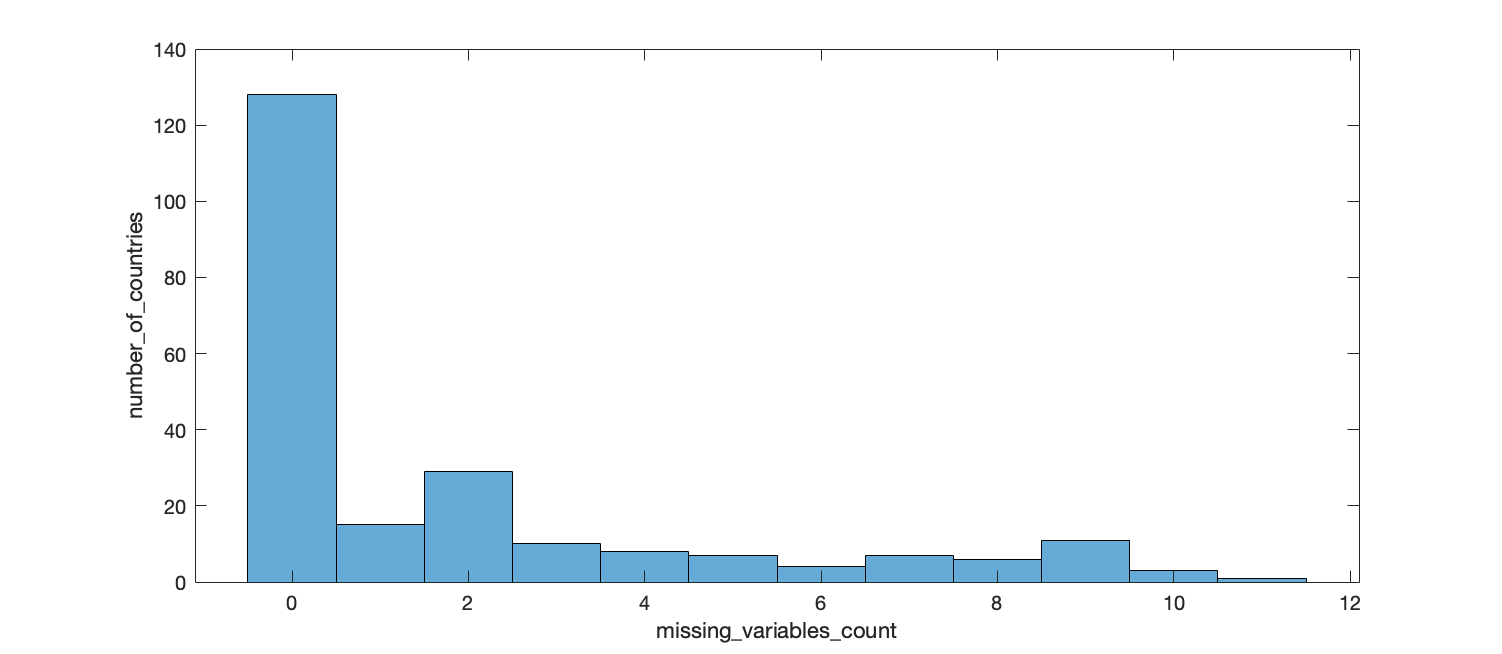
\includegraphics[width=0.85\textwidth]{./images/MissingValues_Country.png}
            \caption{地区数据中各地区的缺失值数量统计}
            \label{images:MissingValues_Country}
        \end{figure}
    \end{minipage}\\\quad\\
    因此,$229$条地区数据中,无缺的只有$128$条,之后如果需要进行聚类分析,需要考虑到此种情况. 如果需要补全数据,只能使用大洲数据的平均补全.
    
      另外,每日数据中包括$21$个地区的有关数据,其中Senegal在地区数据中有数据缺失,遂可以只对余下$20$个地区进行分析,按照大洲分类,分别是
    \vspace{5pt}
    \begin{adjustwidth}{1cm}{0cm}
    {\kaishu
    \begin{itemize}[itemsep=-1pt,topsep=1pt]
        \item [大洋洲:] Australia;
        \item [北美洲:]Canada, United States;
        \item [南美洲:]Chile;
        \item [亚洲:]China, Japan, Malaysia, Saudi Arabia, South Korea, Thailand;
        \item [非洲:]Egypt, Ethiopia, South Africa, Zimbabwe;
        \item [欧洲:]France, Germany, Hungary, Iceland, Sweden.
    \end{itemize}
    }
    \end{adjustwidth}

    \newpage
    %https://max.book118.com/html/2021/0813/6110100143003231.shtm
    \section{长期性分析(自相关分析与周期性特征)}\label{自相关分析}
          本节相关的代码请详见\texttt{./Reports/Chapter4.mlx}. 在这一节,我们尝试解答以下疑问:
        \begin{enumerate}
            \item [1.] COVID-19每日新增病例数据,究竟是一种怎样的时间序列数据?
            \item [2.] 最近有研究指出,SARS-CoV-2更具传染力的新毒株,似乎呈现每隔半年出现一次的周期性,接近其他一些传染病周期性爆发的趋势,这是否能从以上数据中得到某种预见?
        \end{enumerate}
        
          首先,我们必须指出,如果采取十分严厉的管控措施,任何传染病的周期性特征都是可以被人为破坏的,但在目前COVID-19仍旧在世界各地相当盛行的当下,这种可能的周期性是不能被直接排除的选项.

          下面,为了解答上面的疑问,我们以法国的新增病例数据为例,检索部分时段的数据,进行随机性与平稳性检验,以及自回归(ACF)与偏自回归(PACF)分析. 

        \subsection{随机性与平稳性检验}
        首先,可视化出所能获得的全部新增病例数据.\\
\begin{minipage}{\textwidth}
\begin{figure}[H]
    \centering
    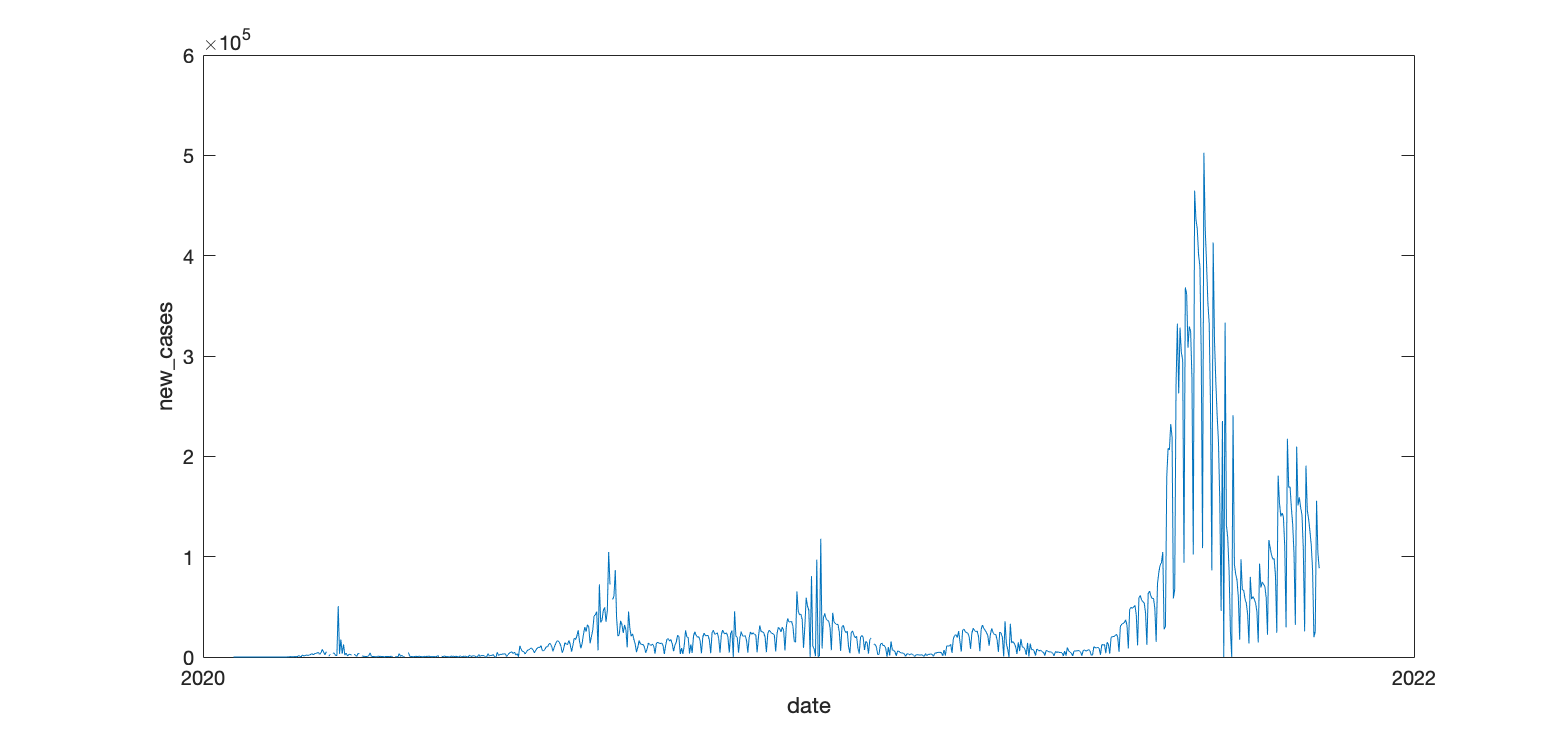
\includegraphics[width=\textwidth]{./images/France_Whole.png}
    \vspace{-3em}
    \caption{法国的全体新增病例数据}
    \label{images:France_Whole}
\end{figure}
\end{minipage}\\\quad\\
从该原始序列的波动变化可以看出,
\begin{enumerate}[itemsep=-2pt,topsep=1pt]
    \item [(1)] 每日新增病例数不是纯随机的;{\kaishu 在MATLAB中,验证非随机性,可以使用\texttt{lbqtest}函数,它使用了Ljung-Box Q统计量;}
    \item [(2)] 长期来看,每日新增病例数总是会有回到$0$的趋势,因此将是平稳的;但短期来看,在病例增长与回落过程中具有趋势性,非平稳;{\kaishu 在MATLAB中,验证平稳性,可以使用内置函数\texttt{adftest}, \texttt{pptest}, \texttt{kpsstest}等检验方式,各自的意义有所不同.}
    \item [(3)] 可能具有长短两种周期性,较短的周期性也可能是由统计方法引起的噪声;{\kaishu 在MATLAB中,进一步的分析将用到后文将使用到的函数\texttt{autocorr}和\texttt{parcorr}.}
\end{enumerate}

    \subsection{自相关分析}
      自相关函数指当日数据与某个时滞数据间的Pearson相关系数,可以理解为当日对某个时滞日间通过各种路径造成的影响力.

      选取第$200$至第$600$条数据,即2020年8月10日至2021年9月14日的数据,利用内置函数\texttt{autocorr},选取较长的时滞期,计算其自回归值,作图如下:\\
    \begin{minipage}{\textwidth}
        \begin{figure}[H]
            \centering
            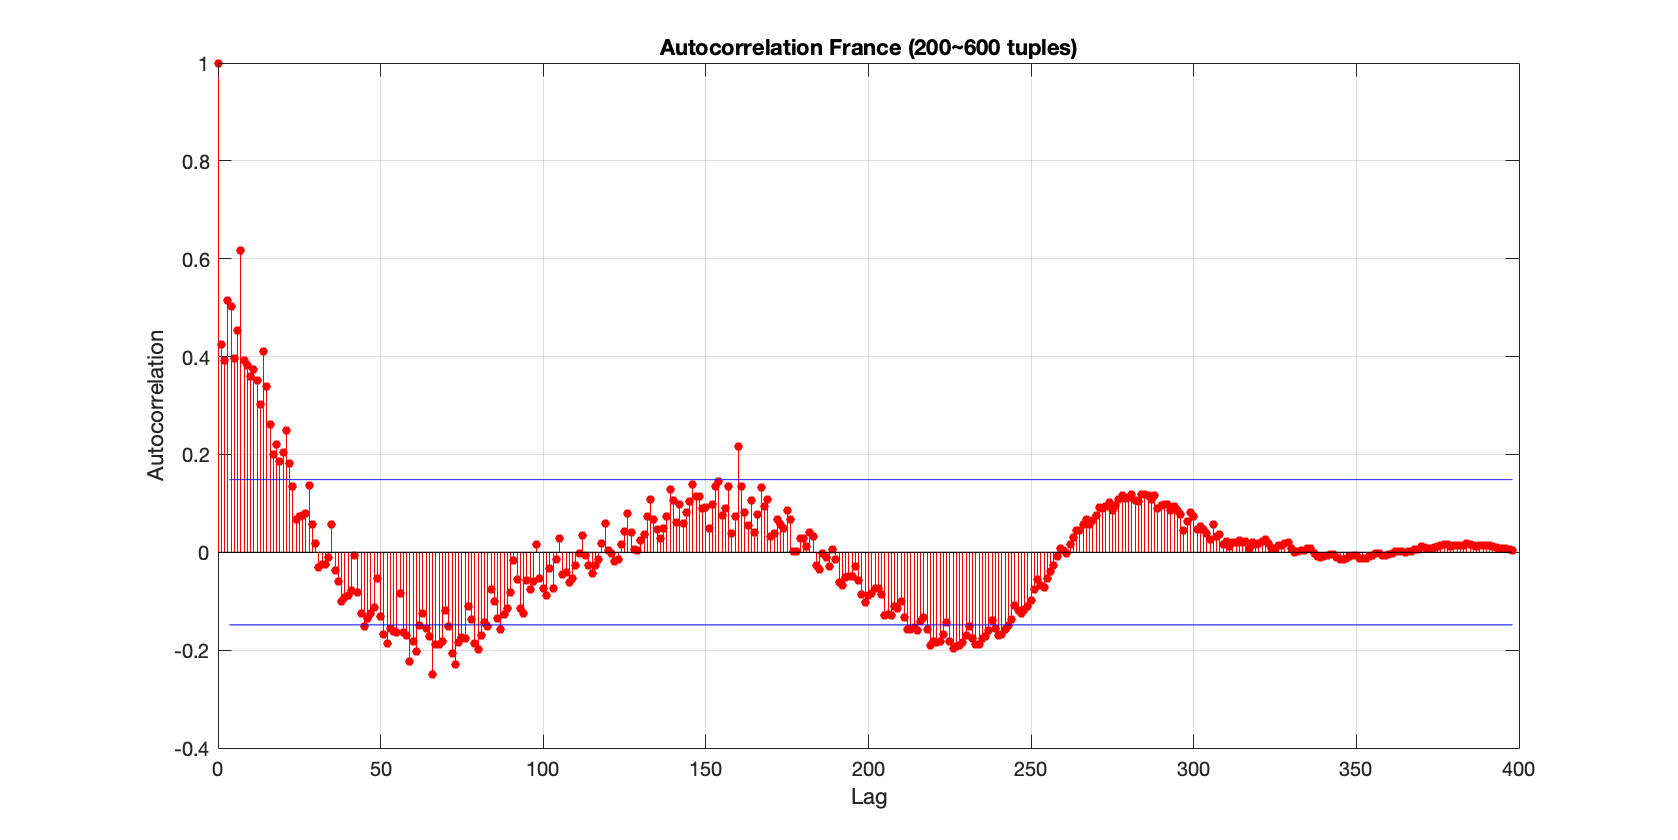
\includegraphics[width=\textwidth]{./images/France_ACF.png}
            \vspace{-3em}
            \caption{法国在一定时期内的自回归值随时滞的变化情况}
            \label{images:France_ACF}
        \end{figure}
    \end{minipage}\\\quad\\
    自相关ACF图呈现波动衰减趋势:(1-) 每隔$150$天左右的时滞,就会出现一个波峰或波谷,它们周期性地逼近乃至突破二倍标准误差带,这暗示新增病例数据可能存在一个$150$天左右的波动周期;(2-) 另外,波动呈现衰减趋势,这暗示可能存在更大的周期;(3-) 波动周期似乎具有缩小的趋势. 但是,也需注意,这里的波峰波谷没有「显著」突破二倍标准误差带,说明其置信仍有待商榷. {\kaishu 注:之所以不选用更临近的数据,是因为临近数据(2022年初)处在病例快速增长期,更具趋势性,会使得ACF图显著拖尾.}

    \subsection{偏自相关分析}
      偏自相关函数可以理解为当日对某个时滞日间通过直接路径造成的影响力,而剔除了其他通过依赖关系造成的影响力. 现在,选用全部数据,利用内置函数\texttt{parcorr},选取较长的时滞期,计算其偏自回归值,作图如下:\\
\begin{minipage}{\textwidth}
    \begin{figure}[H]
        \centering
        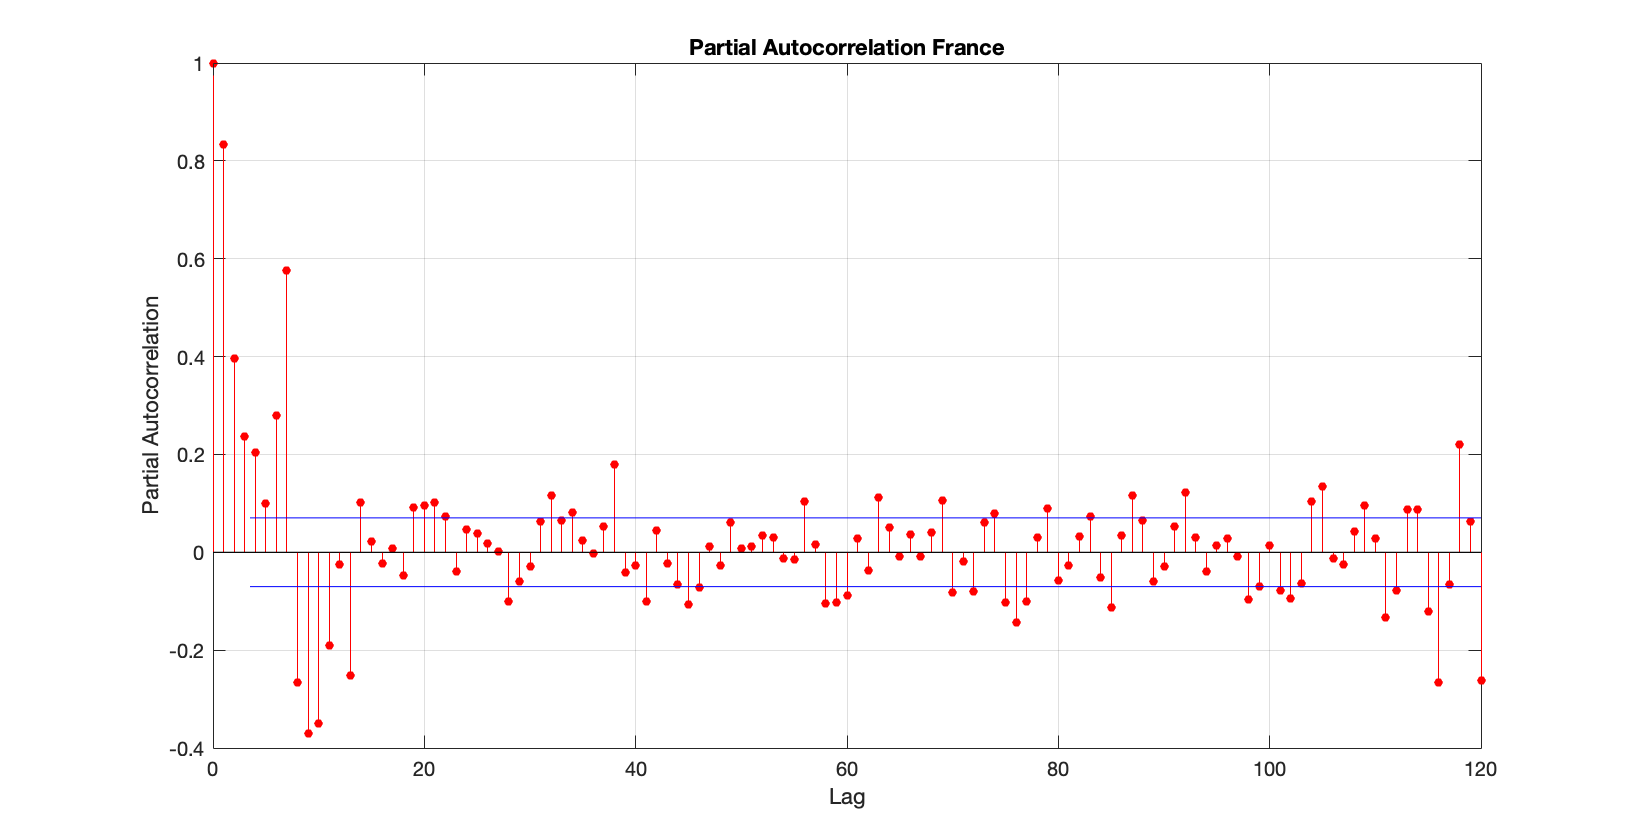
\includegraphics[width=\textwidth]{./images/France_PACF.png}
        \vspace{-3em}
        \caption{法国的偏自回归值随时滞的变化情况}
        \label{images:France_ACF}
    \end{figure}
\end{minipage}\\\quad\\
偏自相关PACF图呈现阻尼振荡式地突破二倍标准误差带,这种正负交变的影响,通常暗示时间序列包含周期性. 另外,从时滞$8$天起,PACF值由正转负,影响力从正相关转向负相关,这与COVID-19的潜伏期长相契合;而从时滞$14$天起,自相关程度开始显著回落至二倍标准误差带以内,有很大的置信认为此时的PACF值与$0$无异,此时相关性衰减到可以不计.

  选取更长的时滞期作图如下:\\
\begin{minipage}{\textwidth}
    \begin{figure}[H]
        \centering
        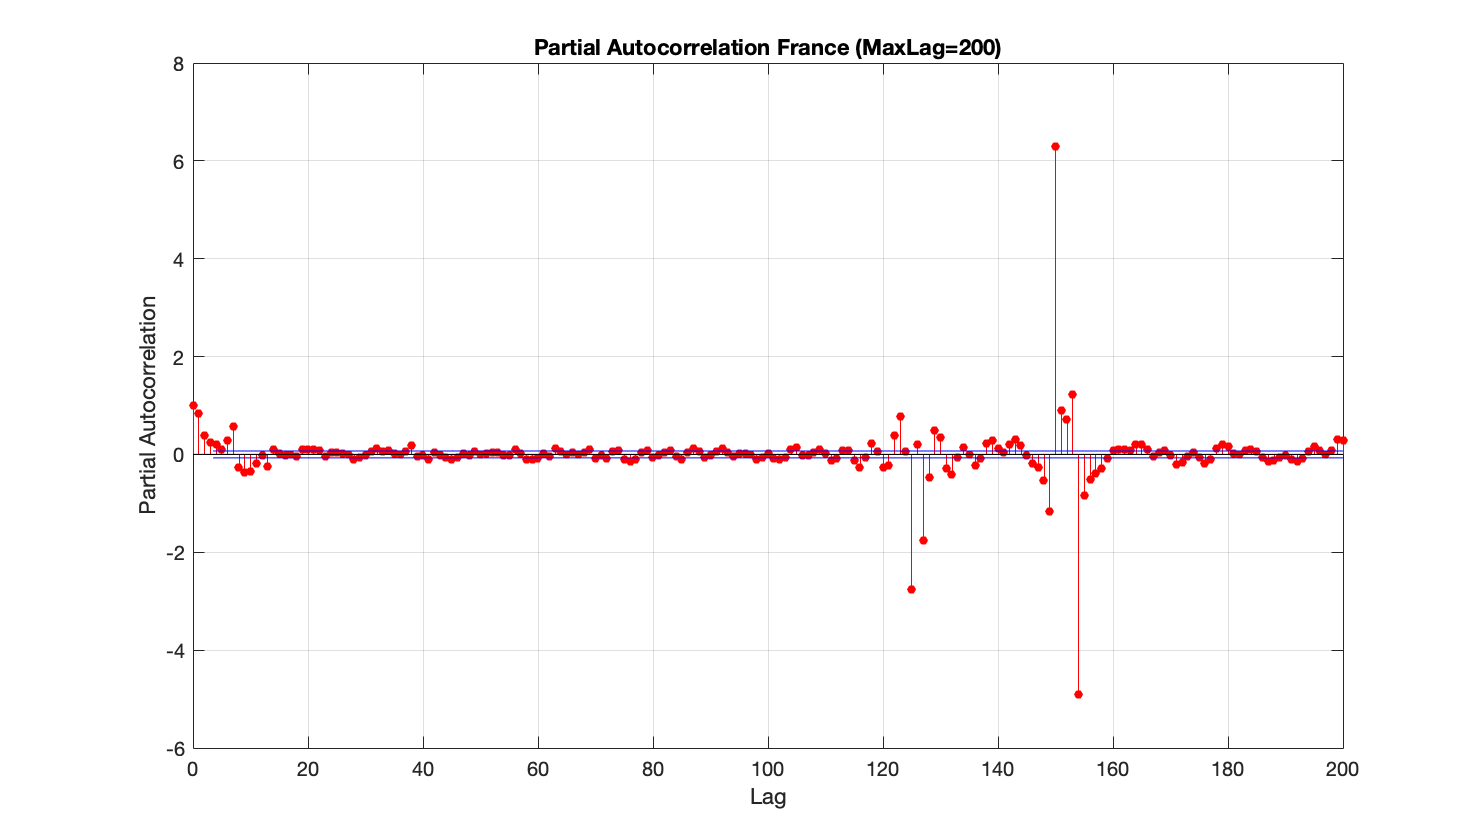
\includegraphics[width=\textwidth]{./images/France_PACF_2.png}
        \vspace{-3em}
        \caption{法国的偏自回归值随时滞的变化情况(MaxLag$=200$)}
        \label{images:France_ACF}
    \end{figure}
\end{minipage}\\\quad\\
更长时滞期的PACF图显示,在时滞$120\sim 160$天时,出现了强烈的正负相关,这暗示了周期性的产生.
\subsection{小结}
  本小节的内容从一个侧面说明了COVID-19新增病例数据,可能存在一种周期性的变化趋势. 传染病形成周期性变化趋势的成因一般有:(1-)传播机制容易实现;(2-)感染后能形成一定免疫力;(3-) 病原体不断发生变异. 而周期性的长短一般取决于:(1-) 感染后免疫水平持续的时间;(2-) 病原体发生变异的速度. 鉴于目前全世界范围内SARS-CoV-2仍在广泛传播与变异,这种周期性于是便成为了一种可能. 我们已经看到的Beta, Delta, Omicron BA.1,2这些亚型的相继爆发,或许正是这种周期性的一种体现. 另外,这里尤须再次指出,严格的管控措施将有效破坏传染病的周期性特征,而周期性正是在这种未能被管控的大环境中所产生的.

  对于呈现周期性变化趋势的时间序列而言,可以进一步开展回归分析,建立回归模型进行长期预测,这对于仍处于SARS-CoV-2各种亚型盛行时期的我们而言,是一个值得研究的领域;只是现时,我们更关注在短期内疫情的发展情况,目的是为了能及时颁布政策进行管控,因此这里不再对长期性多做赘述,下面将进入对短期性的分析.

    \newpage
    \section{短期性分析第一种路径(基于LSTM模型的预测分析)}\label{第一种路径}
      本节相关的代码请详见\texttt{./Reports/Chapter5.mlx}以及\texttt{./src}的相关集成函数.

      前文提到,$229$条地区数据中,无缺的只有$128$条,下面我们就适当补全这些数据,并进行聚类分析. 其次,我们将基于LSTM模型,对每日数据中涉及的$20$个无缺数据地区进行建模,以及预测分析.
    \subsection{聚类分析}
      根据节\ref{数据的缺失值处理}的论述,我们以大洲为界,计算平均值,并附给缺失值. 当然,也可以不作缺失值处理,只对无缺的$128$条地区数据展开分析,或者更进一步地只对每日数据中存在的$20$条地区数据展开分析. 下面我们仍以缺失值处理后的数据为例,并将最后的聚类结果限定在上述$20$个地区.

      其次,我们在开展聚类分析前,先进行了主成分分析,发现了一些地区在某些变量上存在一些离群值,这可能会极大影响后续聚类的结果,比如:
    \begin{enumerate}[itemsep=-2pt]
        \item [(1-)] 在人口变量上,中国和印度比较突出;
        \item [(2-)] 在人口密度变量上,日本和韩国等地区比较突出;
        \item [(3-)] 在心血管疾病死亡率变量上,埃及等地区比较突出. 
    \end{enumerate}
    由于人口的多寡对于疫情的发展而言,并没有人口密度来得重要,因此我们进一步剔除了人口变量,但对于其余这些变量,虽然方差较大,但我们认为它们对疫情发展的相关性也较大,于是进行了保留. 
    
      另外,我们还将男性吸烟率与女性吸烟率取了平均值,因为我们认为,对于疫情发展而言,男女性别所造成的地区差别并不相关. 如此之后,主成分分析后的第一个主成分仍达到了$99.06\%$的信息占比,我们认为这可能是人均GDP数据方差较大所引起的结果,但是我们认为人均GDP数据与疫情发展的相关性还是很大的,所以我们保留了这个变量. 值得注意的是,先前我们所作的平均值赋值可能因此降低了一些变量的方差,使得主成分分析更偏爱其他的一些变量,我们认为,从节\ref{数据的缺失值处理}中我们已经看到各个变量的缺失个数是相当的,对最后结果的影响不会很大. 最后,我们选取主成分分析后的\textbf{前$5$个成分}进行随后的聚类分析. 

      再次,我们选取了$k$-mean方法进行聚类. 我们利用\textbf{肘部原理}确定最佳的$k$值,我们计算$k$取$1$至$10$时每种各$10$次结果的平均值,对其误差作图,如下所示.\\
    \begin{minipage}{\textwidth}
        \begin{figure}[H]
            \centering
            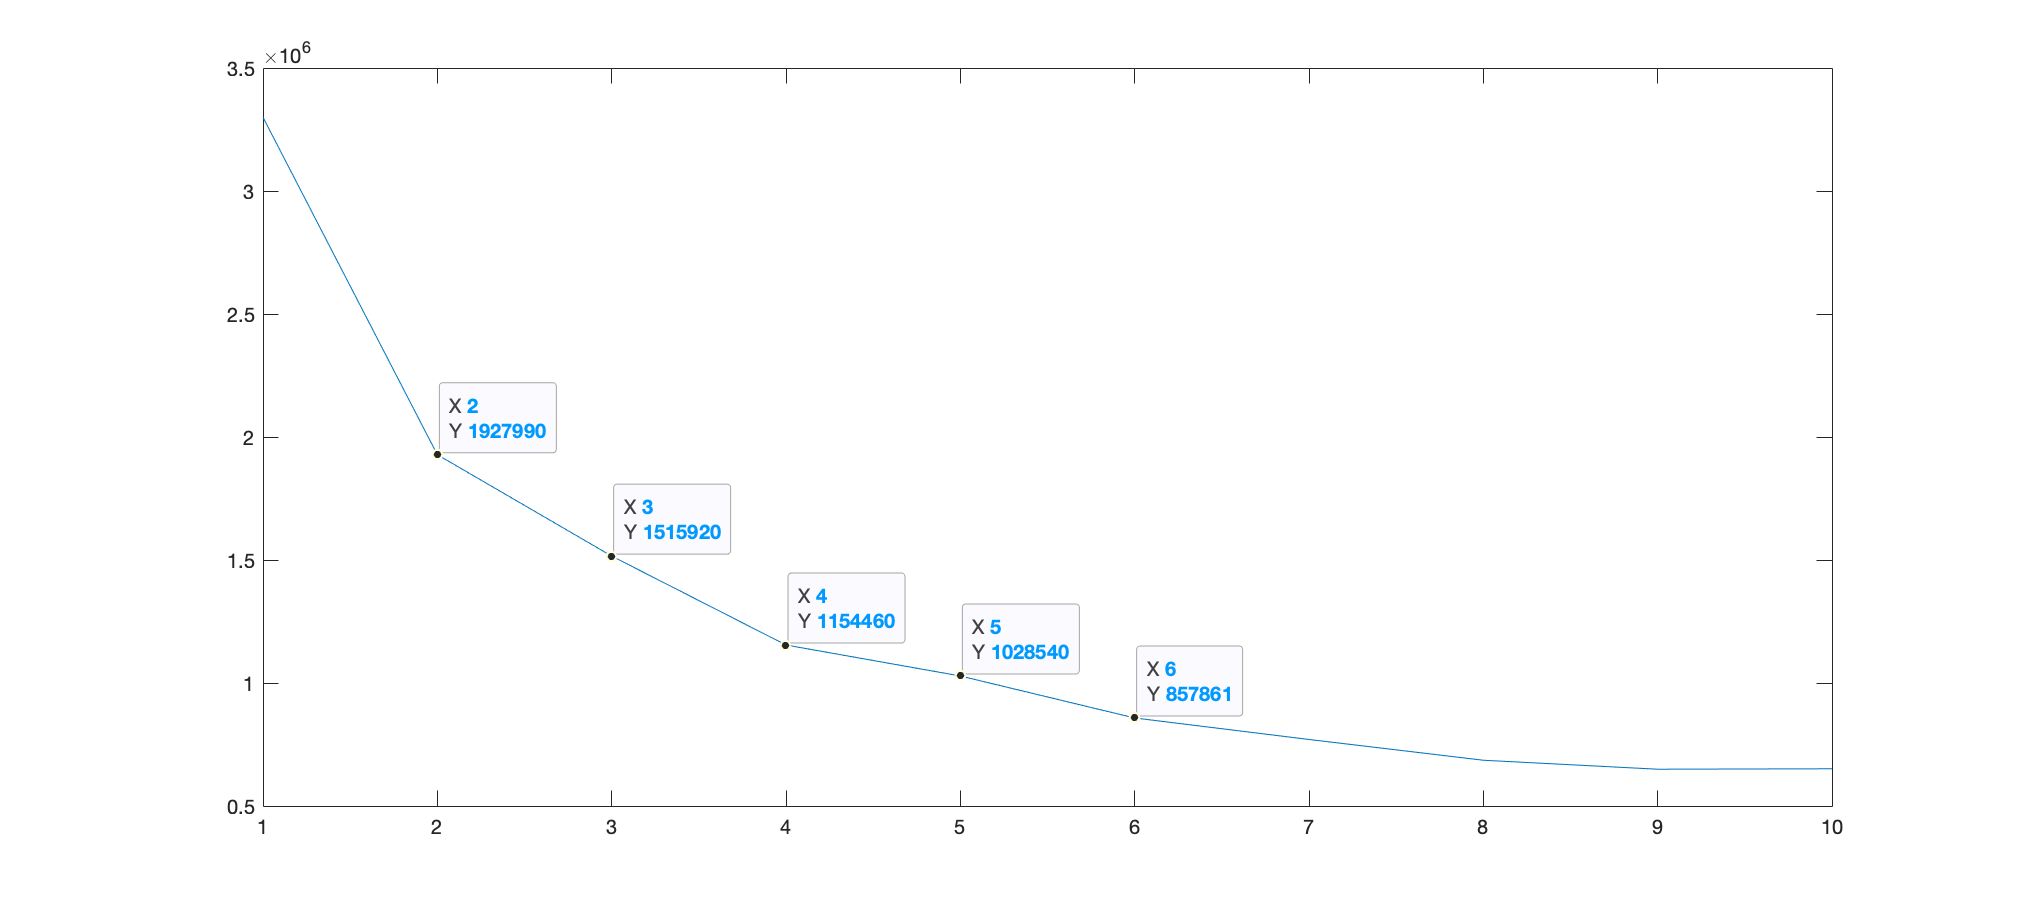
\includegraphics[width=0.9\textwidth]{./images/Elbow.png}
            \vspace{-1.5em}
            \caption{利用肘部原理确定$k$值}
            \label{images:Elbow}
        \end{figure}
    \end{minipage}\\\quad\\
    图中,我们认为最快下降处出现在$k=4$附近. 于是我们将地区数据中的地区划分为$4$类,并将某一次的分类结果如下所示.\\
    \begin{minipage}{\textwidth}
        \begin{figure}[H]
            \centering
            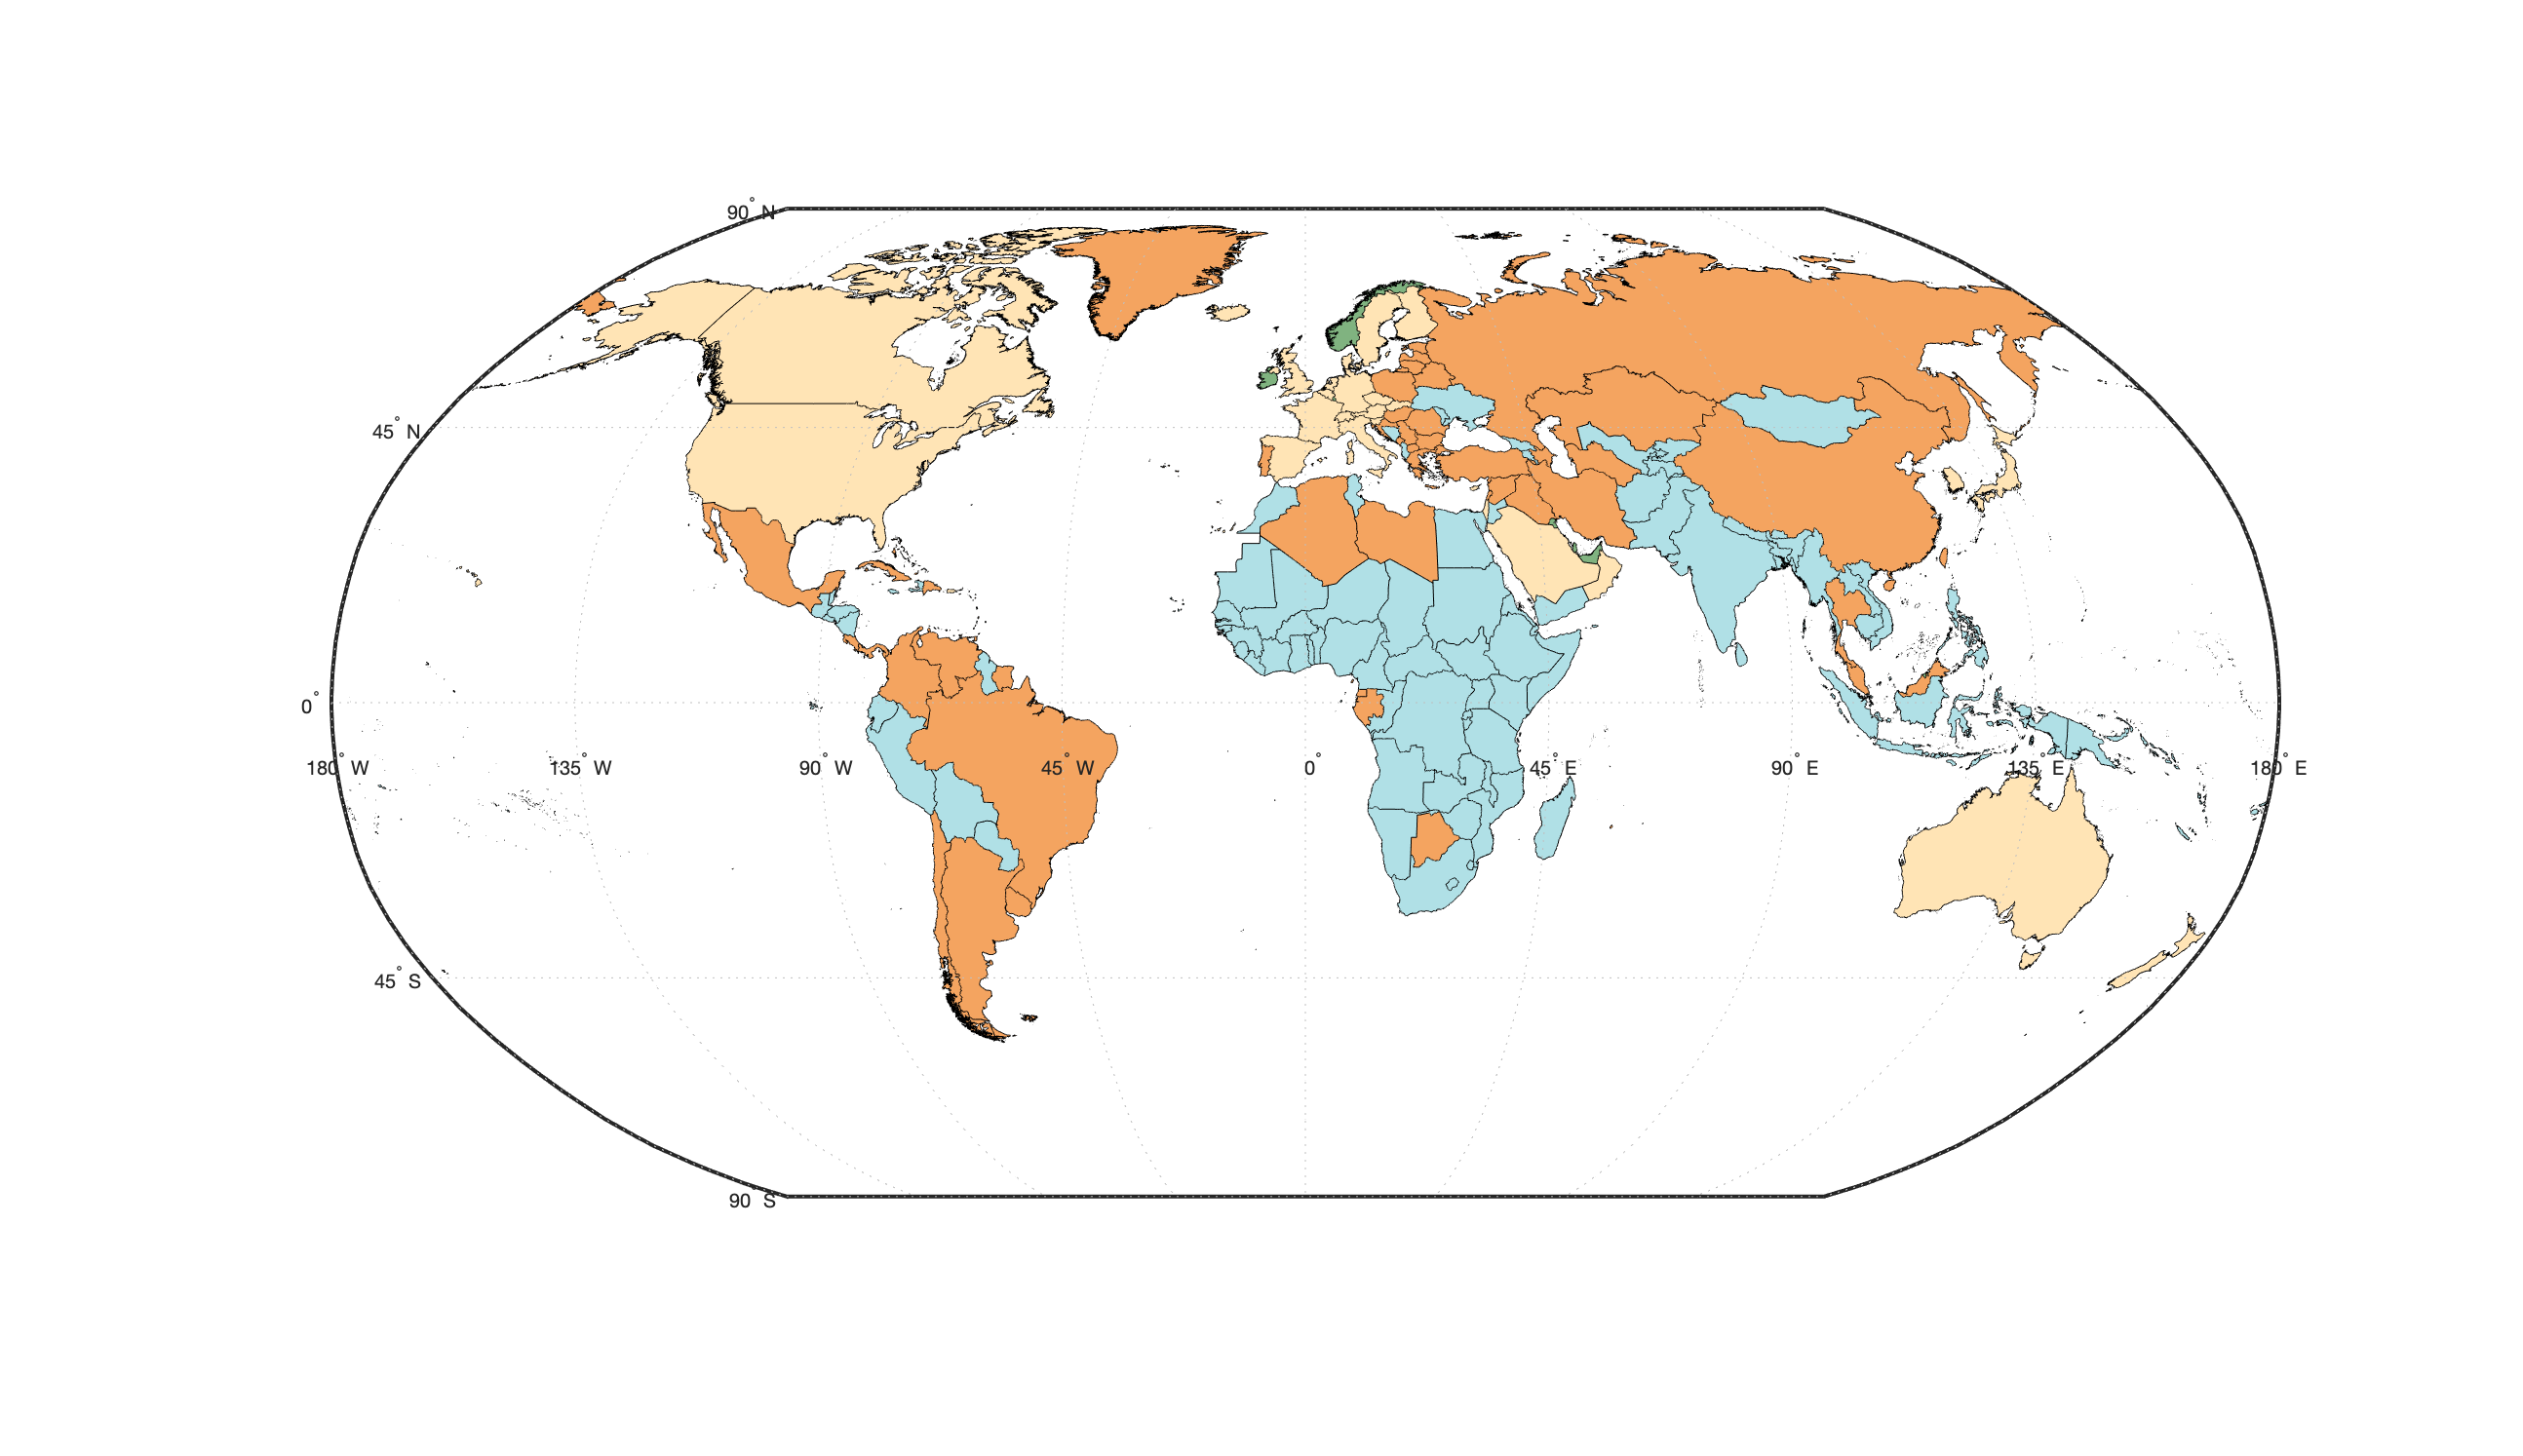
\includegraphics[width=0.9\textwidth]{./images/World_Classification.png}
            \vspace{-3em}
            \caption{$4$-mean分类结果}
            \label{images:World_Classification}
        \end{figure}
    \end{minipage}\\\quad\\
    
      在后面的小节中,我们将只考虑每日数据中出现的无缺的$20$个地区的数据,我们将某一次的分类结果记录如下:
    \vspace{5pt}
    \begin{adjustwidth}{0.6cm}{0cm}
    \begin{itemize}
        \item [第一类:] Ireland;
        \item [第二类:] Australia, Canada, France, Germany, Iceland, Japan, Saudi Arabia, South Korea, Sweden, United States;
        \item [第三类:] Chile, China, Hungary, Malaysia, Thailand;
        \item [第四类:] Egypt, Ethiopia, South Africa, Zimbabwe.
    \end{itemize}
    \end{adjustwidth}
    \vspace{5pt}
    \subsection{构建模型}
	\subsubsection*{简单的情形(对分类的检验,使用神经网络的可行性)}
	  上面我们已经给出了聚类分析. 自然地,我们想要继续探究,我们的分类是否正确地指导了我们对于疫情的解读? 出于此目的,我们使用了MATLAB的神经网络工具箱,因而可以较为简单地搭建出一个网络,其网络结构用 MATLAB 的格式简单地例举如下.
	\begin{align*}
		&\texttt{sequenceInputLayer(8)}\\
    	\rightarrow\quad&\texttt{fullyConnectedLayer(300)}\\
    	\rightarrow\quad&\texttt{reluLayer}\\
    	\rightarrow\quad&\texttt{fullyConnectedLayer(300)}\\
    	\rightarrow\quad&\texttt{reluLayer}\\
    	\rightarrow\quad&\texttt{fullyConnectedLayer(300)}\\
    	\rightarrow\quad&\texttt{reluLayer}\\
    	\rightarrow\quad&\texttt{fullyConnectedLayer(numResponses)}\\
    	\rightarrow\quad&\texttt{regressionLayer}
	\end{align*}
	它将用于预测每日新增病例的变化情况. 我们传入的数据的字段包括
	\[
	\begin{bmatrix}
		\text{当前总感染人数}\\
		\text{前4日新增人数}\\
		\text{前3日新增人数}\\
		\text{前2日新增人数}\\
		\text{前1日新增人数}\\
		\text{PCA 截断值1}\\
		\text{PCA 截断值2}\\
		\text{PCA 截断值3}
	\end{bmatrix},
	\]
	用于对后一日的新增病例个数进行预测. 这里,我们对新增病例数进行了光滑:记新增病例数所称的向量为$\mathcal{N}$,我们作了如下光滑
	\[
		\mathcal{N}_{\mathcal{S}} = \text{conv}(\mathcal{N},\mathcal{K}), \quad \mathcal{K} = \begin{bmatrix}
			\displaystyle\frac{1}{4}&\displaystyle\frac{1}{4}&\displaystyle\frac{1}{4}&\displaystyle\frac{1}{4}
	\end{bmatrix}.
	\]

	  我们以前文分类中第二类的部分地区为例,包括France, South Korea, Australia, Canada, Iceland,对这些地区的数据,采用Adam 优化器,训练 4000 个 回合数. 选取的用于验证的地区为 Saudi Arabia, Germany, Japan, United States. 初始的学习率设置为 $0.001$,并每 75 个 epoch 乘以 $0.95$.

	  为了说明我们的网络是工作的,我们先给出其在训练集上的效果:\\
    \vspace{-1em}
    \begin{minipage}{\textwidth}
        \begin{figure}[H]
            \centering
	        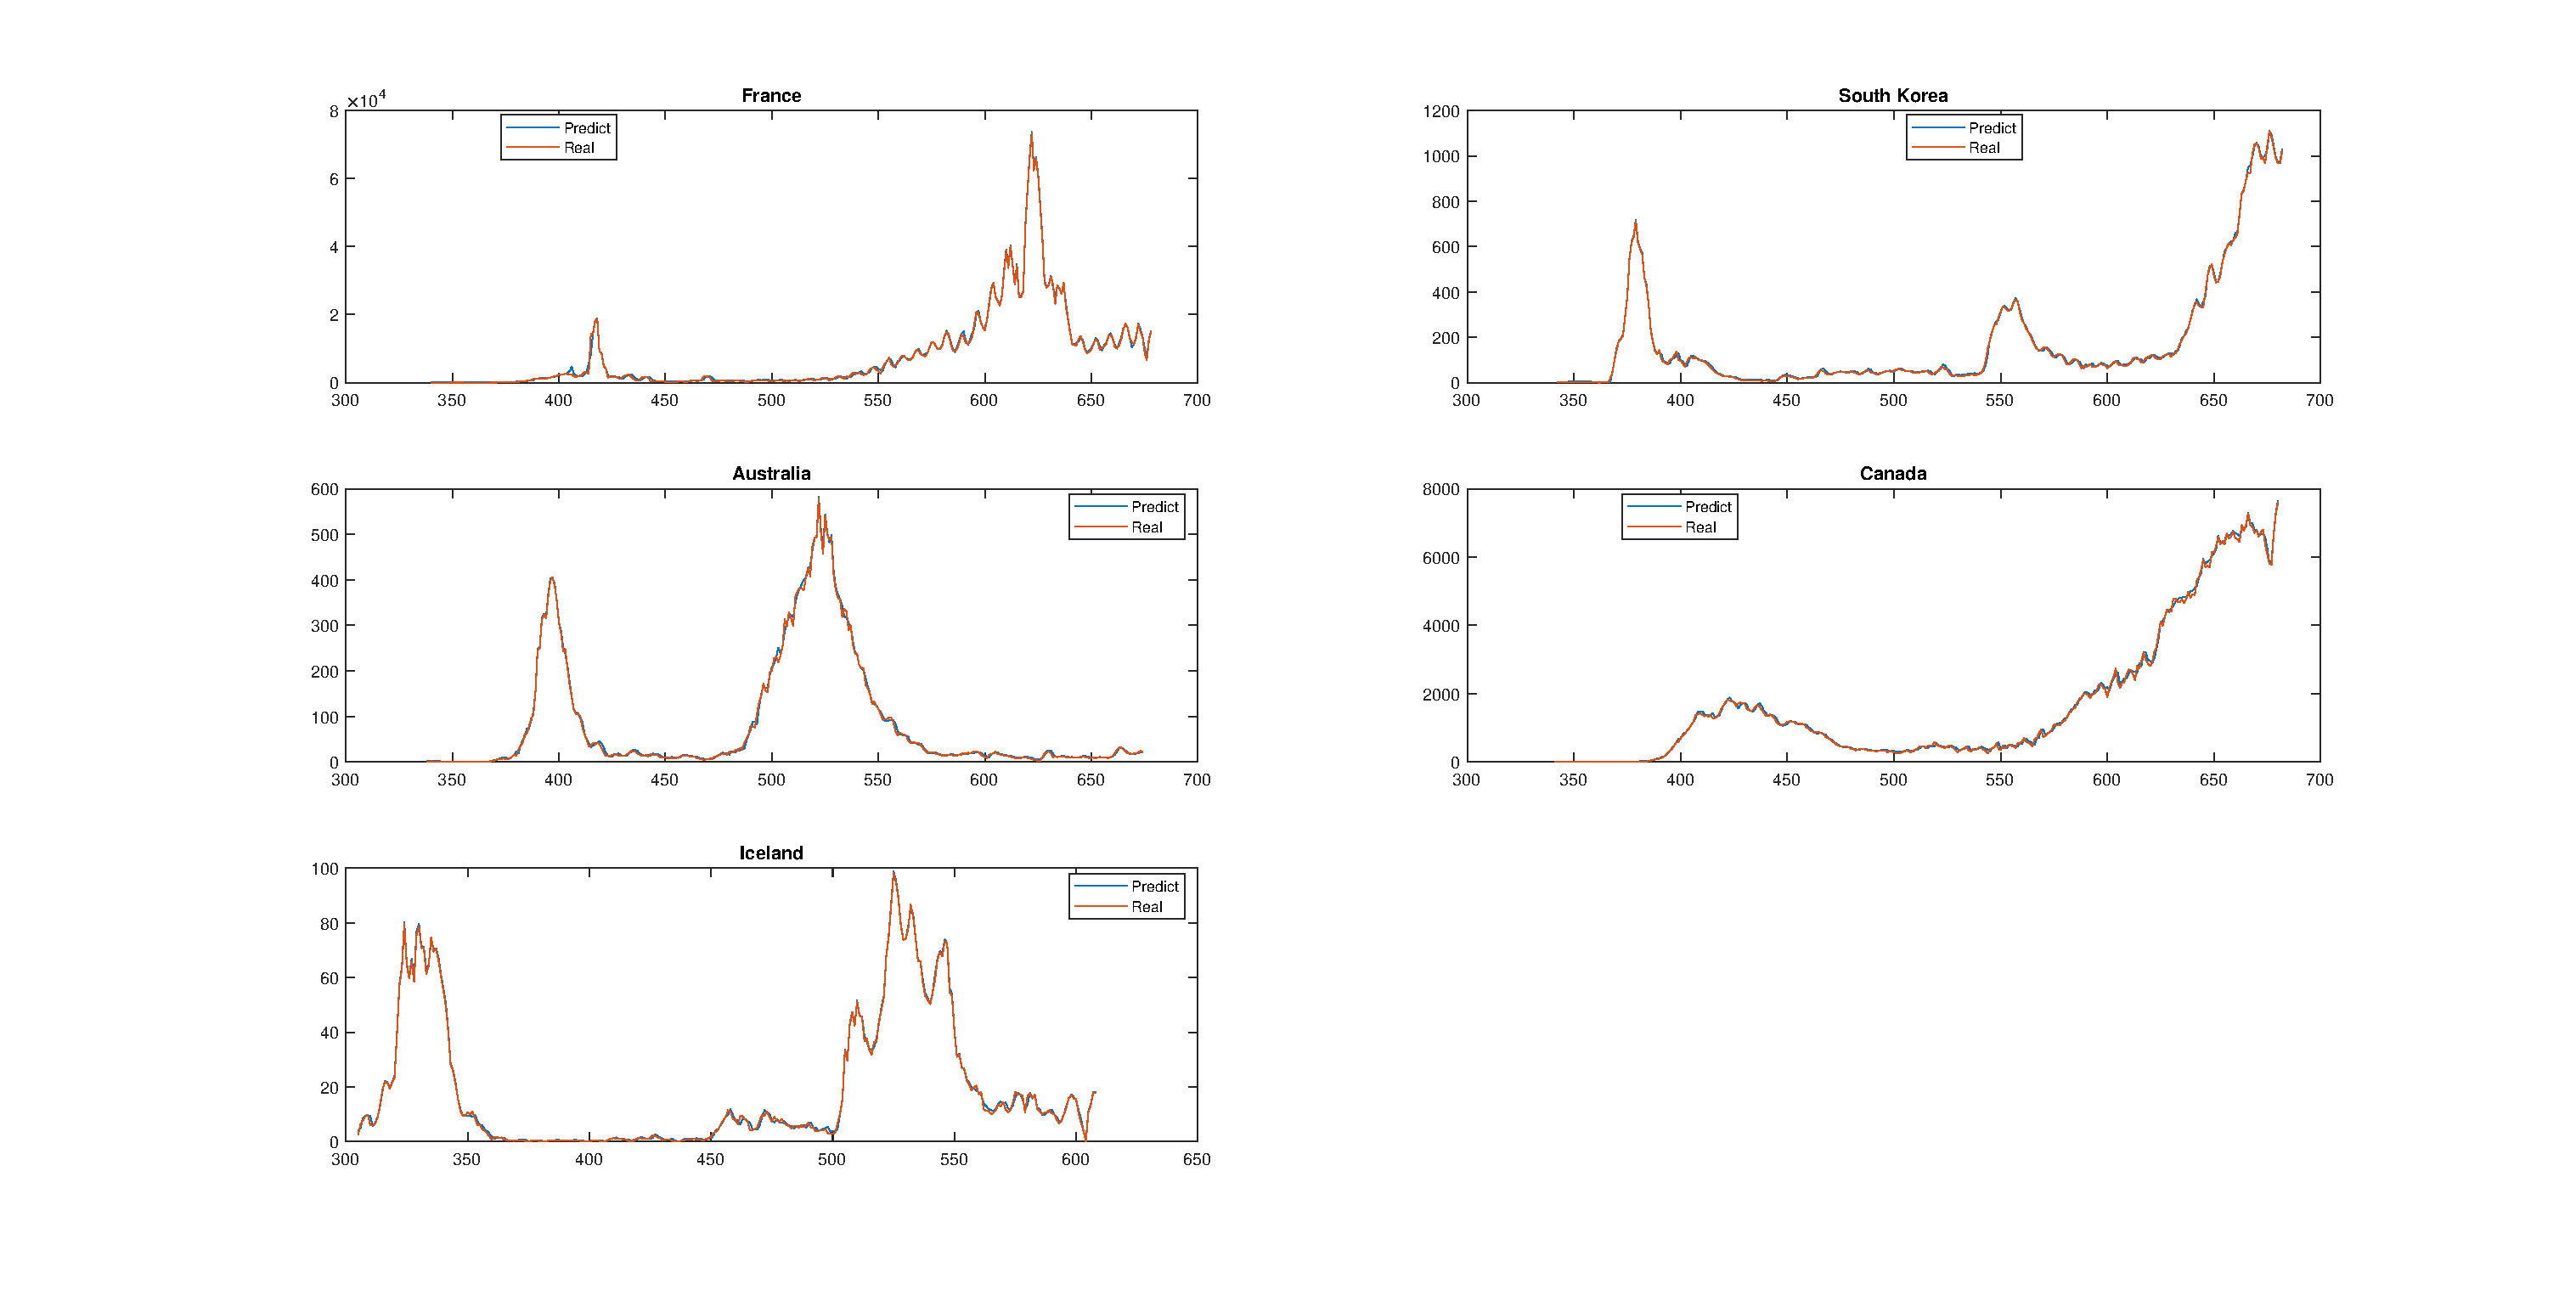
\includegraphics[height=12cm, width=14cm]{./Chap4/trainset.eps}
            \vspace{-2em}
            \caption{神经网络在训练集上的效果图}
	    \end{figure}
    \end{minipage}\\\quad\\
    \subsection{预测分析}
        \subsubsection{简单情形的预测分析}
	  对于测试集,我们选取 Saudi Arabia, Germany, Japan, United States 四个地区. 所得到的预测结果见下图:\\
	\begin{minipage}{\textwidth}
        \begin{figure}[H]
            \centering
            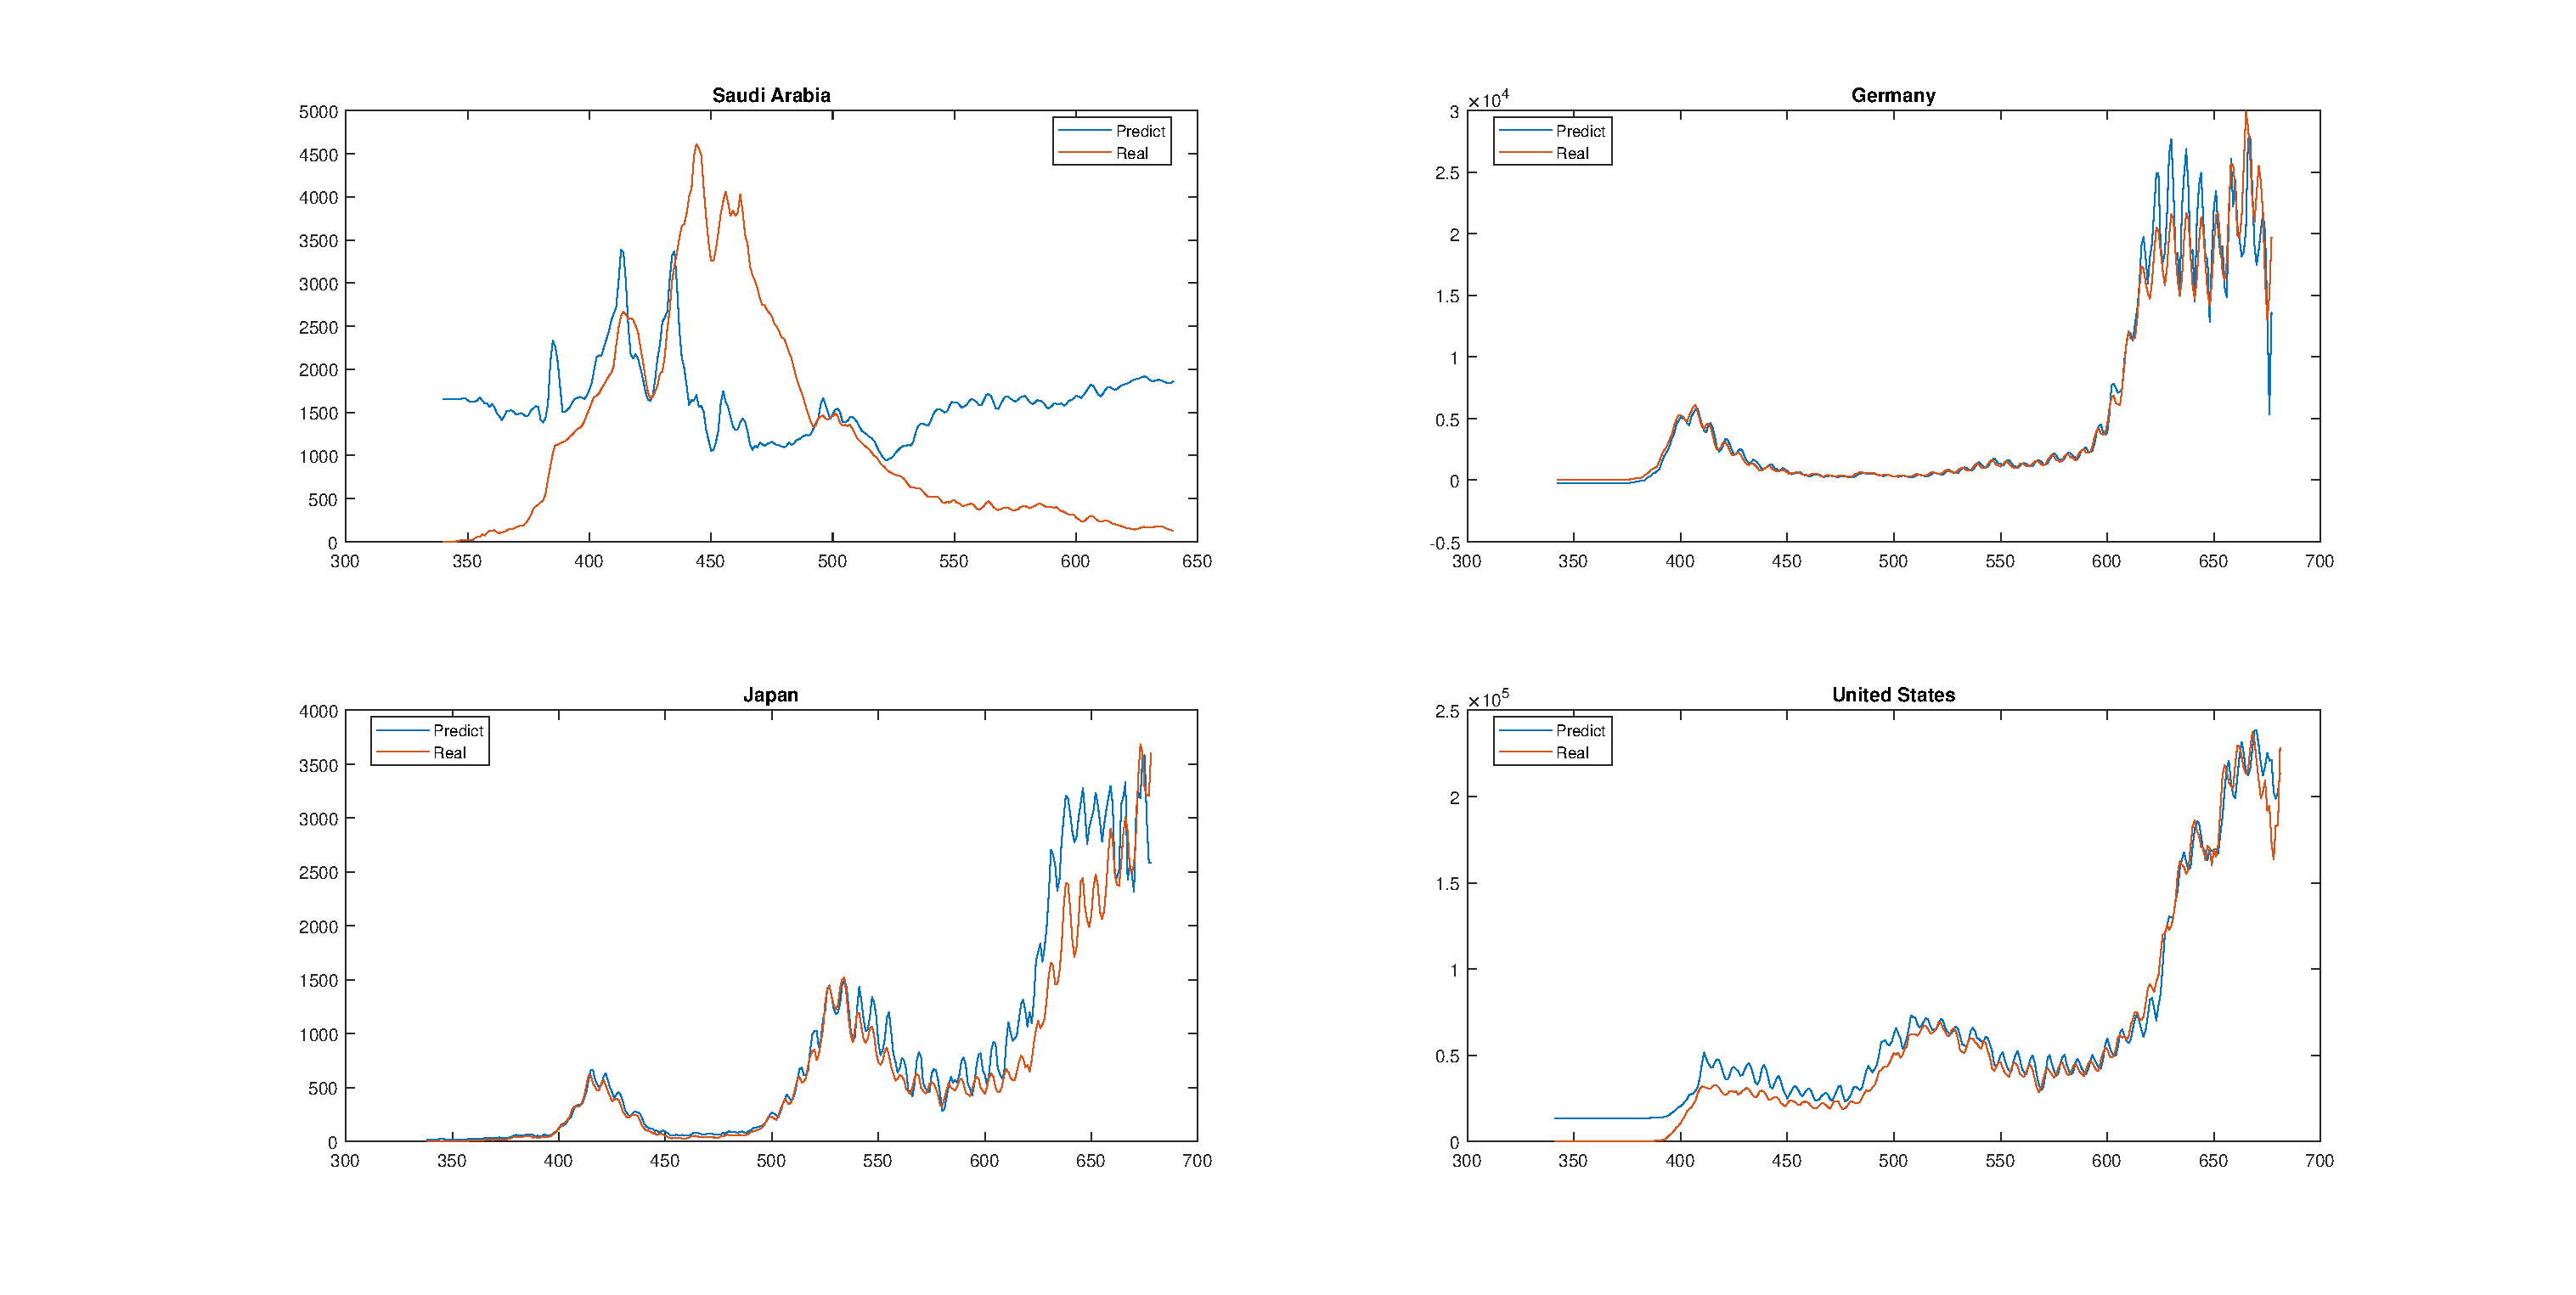
\includegraphics[height=8cm, width=14cm]{./Chap4/Pred2.eps}
            \vspace{-1.5em}
            \caption{神经网络在测试集上的效果图}
        \end{figure}
    \end{minipage}\\\quad\\
	从中可以看到,除了 Saudi Arabia 以外,其余地区的拟合状况都是不错的; 注意到 Saudi Arabia 的疫情曲线也明显与其余几个地区有差别. 这一方面说明我们对地区的分类并不能完全说明其疫情的发展,另外一方面说明我们的网络是 data-driven 的: 在并未见过这样疫情发展的情况下,难以做出准确的预测. 如果我们在训练集中加上 China, Ethiopia, Zimbabwe 三个地区,得到的结果将会有相当大的改善:\\
    \vspace{-1em}
    \begin{minipage}{\textwidth}
        \begin{figure}[H]
            \centering
	        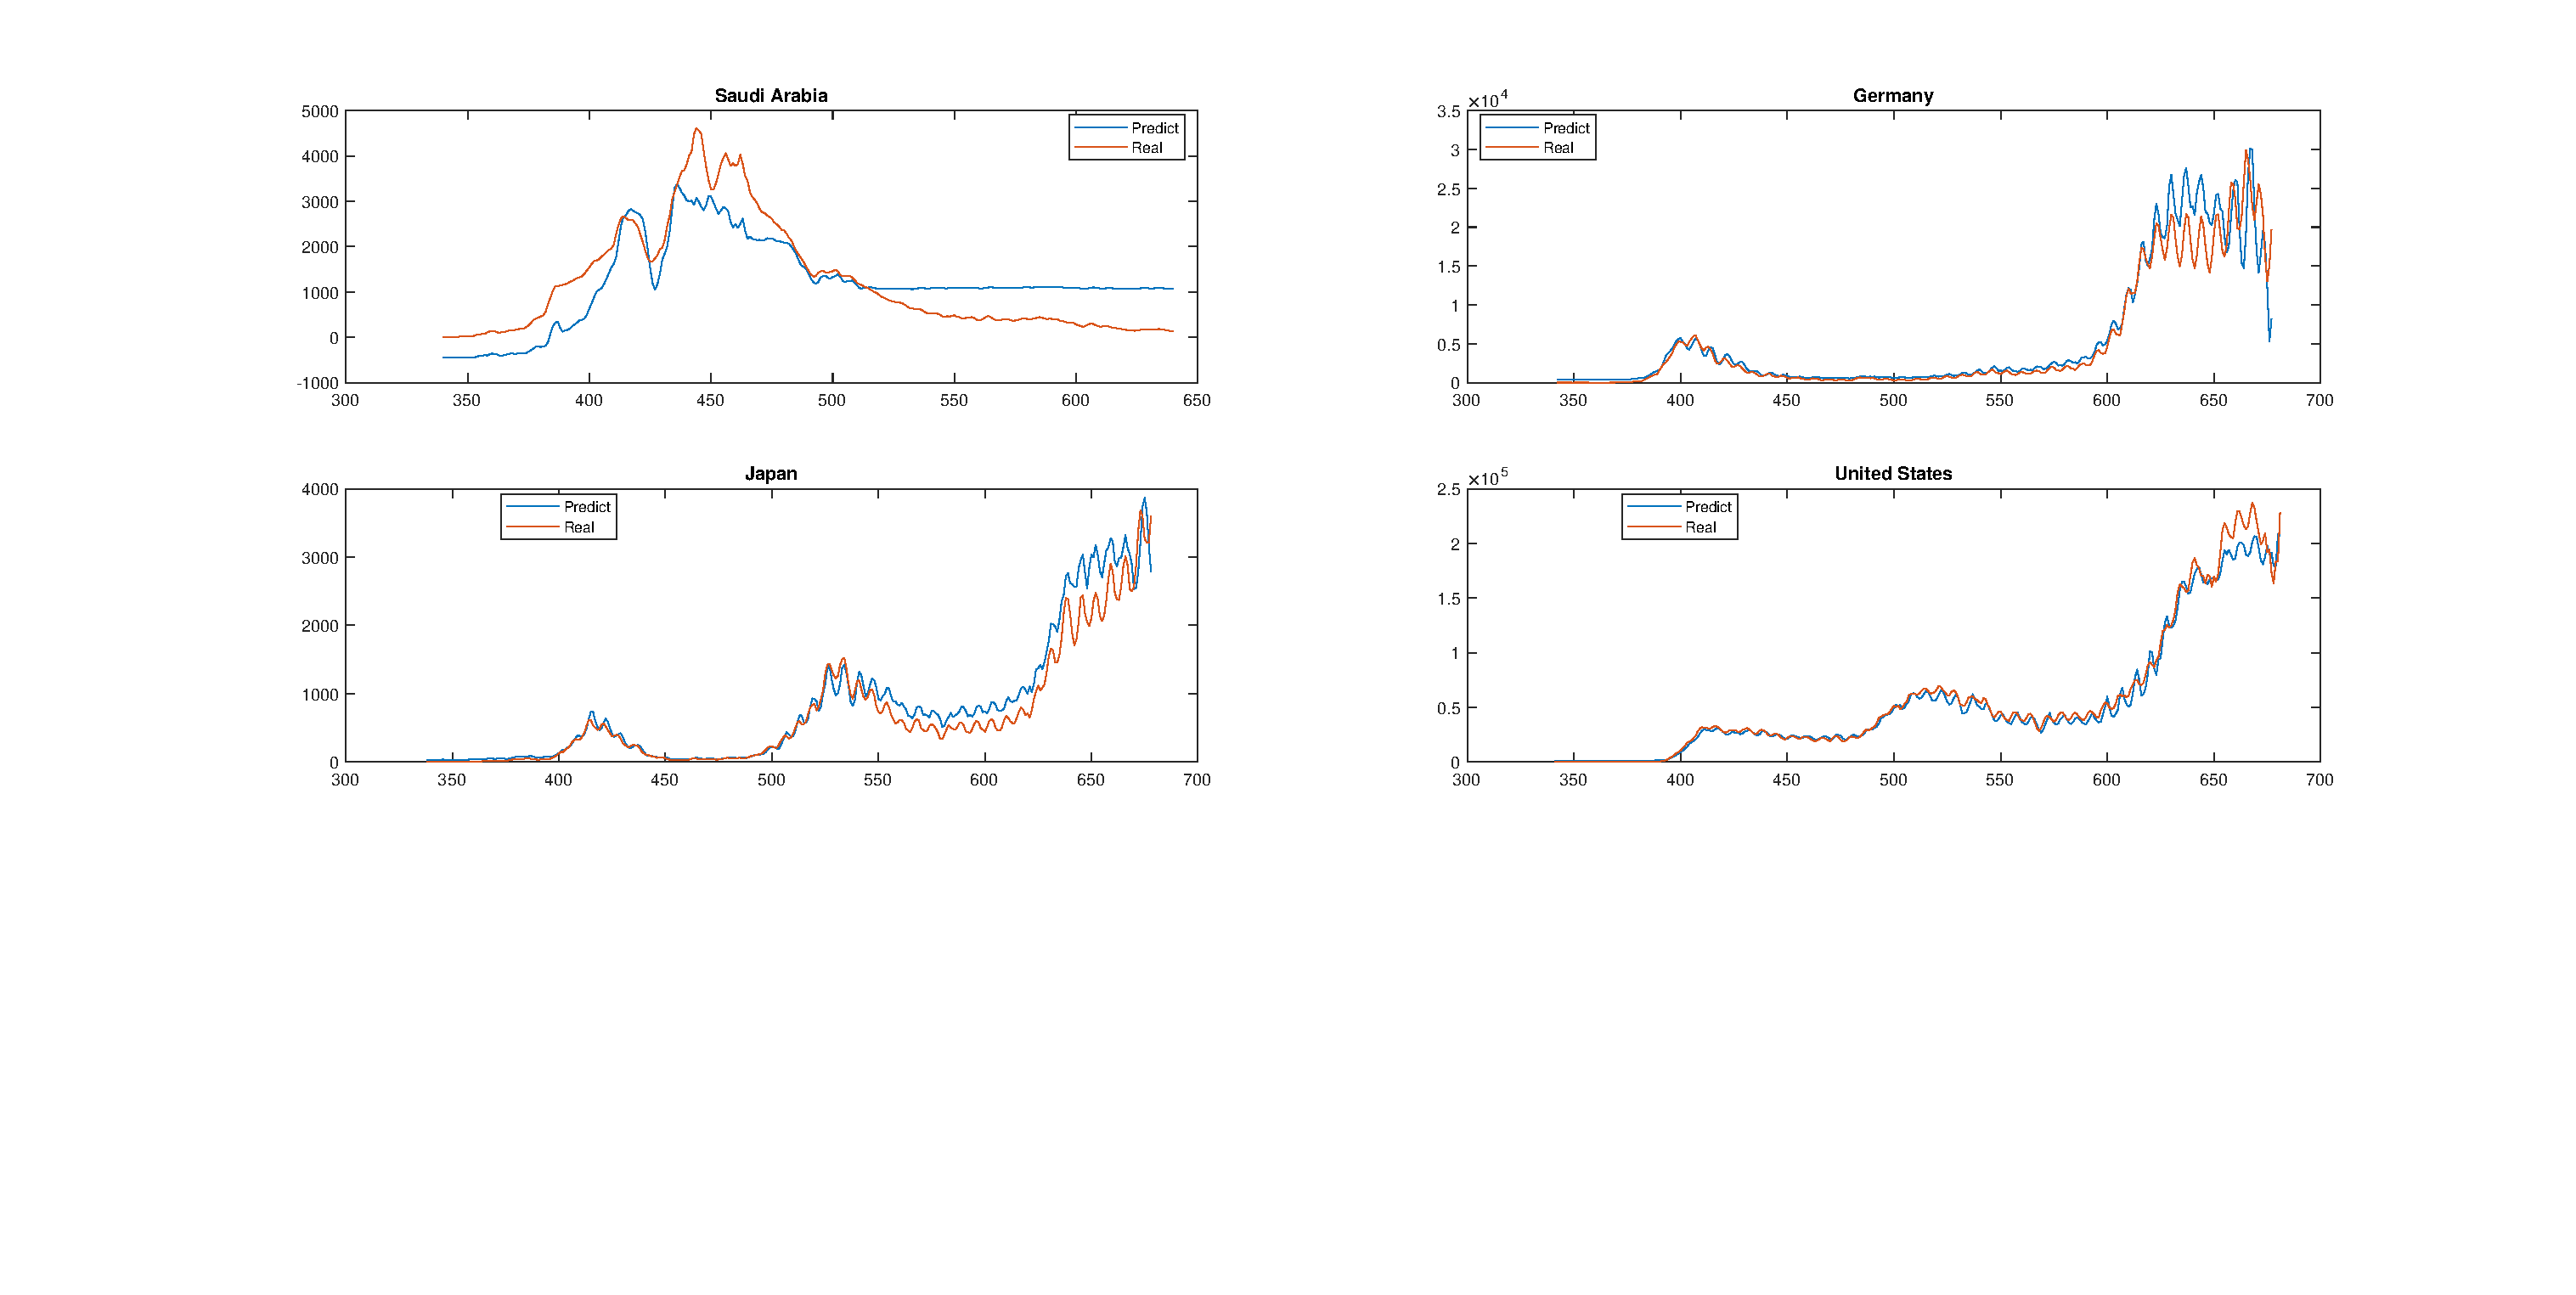
\includegraphics[height=12cm, width=14cm]{./Chap4/Pred3.eps}
            \vspace{-4cm}
            \caption{神经网络在测试集上的效果图2}
        \end{figure}
    \end{minipage}\\\quad\\
    \quad\\
	所以我们可以预见的是,在数据越多的情况下,我们能越好地预测疫情的发展状况.

	\subsubsection{LSTM: 预测疫情发展状况}
      注意到在本次作业中,并没有无症状携带者,易感人群,死亡病例等数据,所以这里传统的 SEIR 或者 SEIRS 模型并不适用. 而新增病例是与时间有很强关系的数据,我们选择 RNN 来进行预测是自然的. 这里我们选择 RNN 中的特殊种类——LSTM 进行预测. 同样地,为方便起见,也与 MATLAB 的风格相符,我们直接列出网络结构:
	\begin{align*}
		&\texttt{sequenceInputLayer(8)} \\
        \rightarrow\quad&\texttt{fullyConnectedLayer(30)}\\
    	\rightarrow\quad&\texttt{reluLayer}\\
    	\rightarrow\quad&\texttt{lstmLayer(400)}\\
    	\rightarrow\quad&\texttt{reluLayer}\\
    	\rightarrow\quad&\texttt{fullyConnectedLayer(30)}\\
    	\rightarrow\quad&\texttt{reluLayer}\\
    	\rightarrow\quad&\texttt{fullyConnectedLayer(numResponses)}\\
    	\rightarrow\quad&\texttt{regressionLayer}
	\end{align*}

      首先,我们从不同的类别中挑出几个有代表性的地区,这里我们的选取是 China, France, Ethiopia, Zimbabwe, Hungary, South Korea, Egypt, Australia, Canada, Iceland. 我们选取 Adam 优化器,对上述数据训练 2000 个 epoches. 初始的学习率设置为 $0.001$,并每 75 个 epoch 乘以 $0.95$. 同样地记新增病例数所称的向量为 $\mathcal{N}$,我们使用
	\[
		\mathcal{N}_{\mathcal{S}} = \text{conv}(\mathcal{N},\mathcal{K}), \quad \mathcal{K} = \begin{bmatrix}
			\displaystyle\frac{1}{4}&\displaystyle\frac{1}{4}&\displaystyle\frac{1}{4}&\displaystyle\frac{1}{4}
	\end{bmatrix}
	\]
	  我们将每日新增病例数与上面的核进行卷积,考虑是两方面的: 一是为了方便网络的训练,二是用四天的数据的平均来代替某一天的数据.
	在得到的数据中,我们将前 $\frac{4}{5}$ 的病例数作为训练集,将后 $\frac{1}{5}$ 的数据作为测试集. 可以看到效果是很好的.\\
    \vspace{-1em}
    \begin{minipage}{\textwidth}
        \begin{figure}[H]
            \centering
	        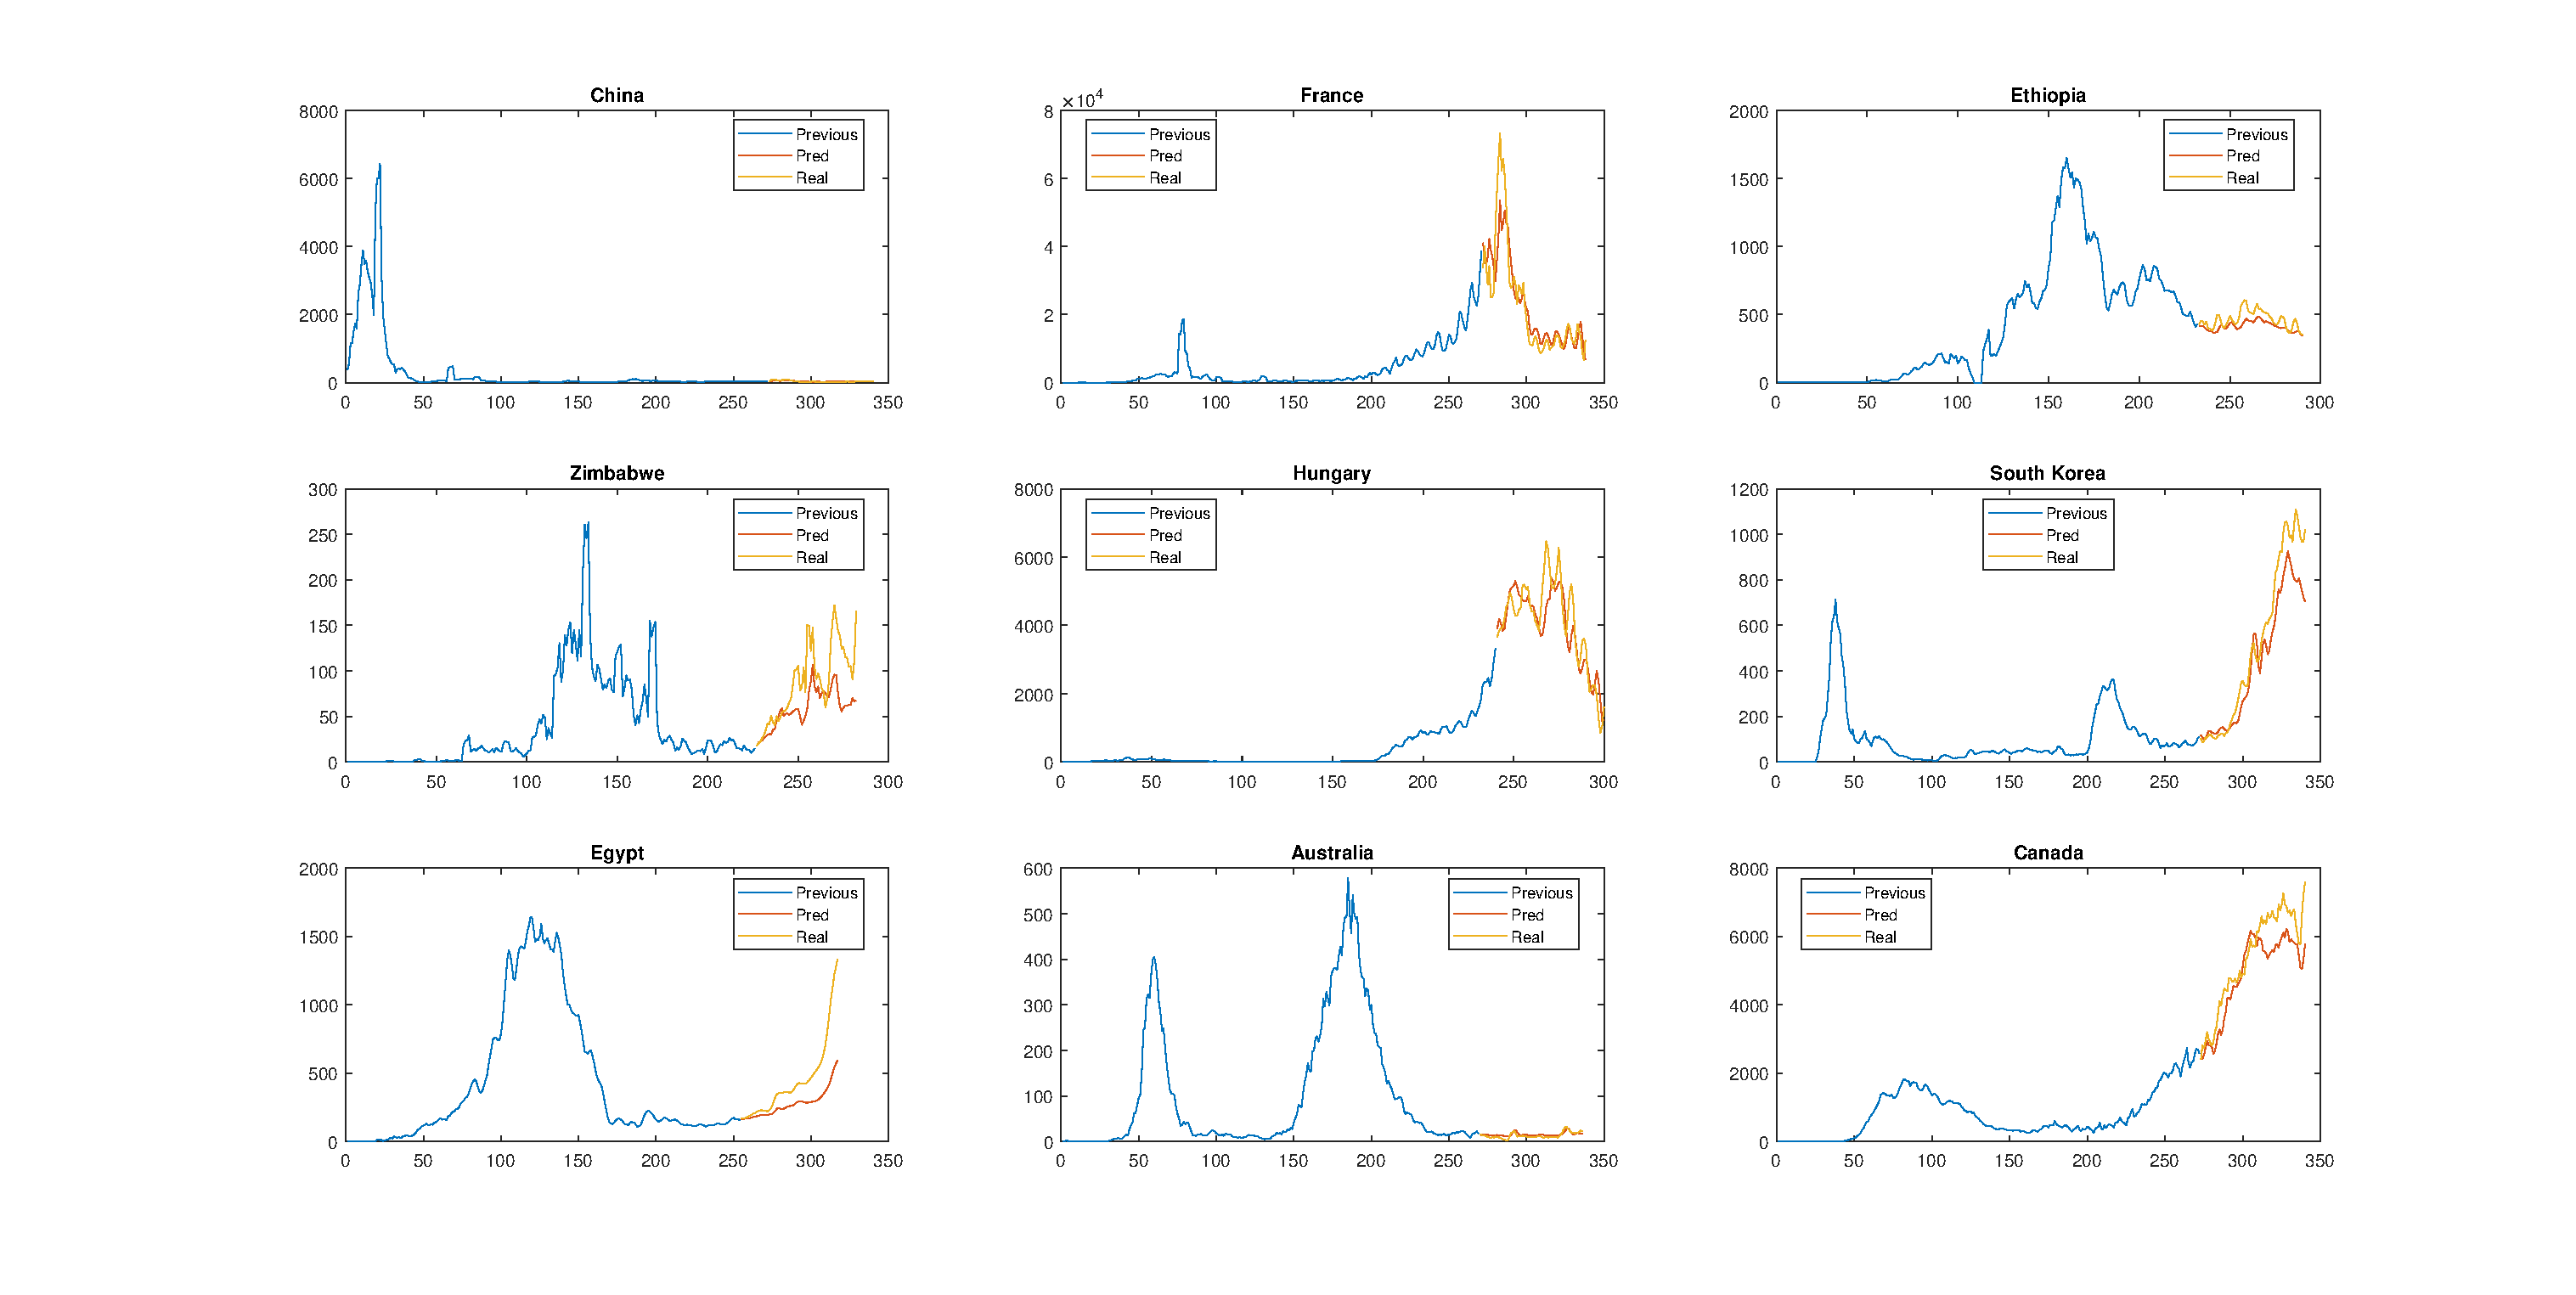
\includegraphics[height=8cm, width=10cm]{./Chap4/Pred.eps}
            \vspace{-1.5em}
            \caption{测试效果}
	\end{figure}
    \end{minipage}\\\quad\\
	  这时我们相当于使用一个地区过去的疫情的发展信息来预测未来的发展. 我们想要看这个网络是否学到的是使用过去的信息,抑或如果是没有见过的情况,就难以处理? 注意到我们上面给出的例子,我们使用 France, South Korea, Australia, Canada, Iceland 进行训练,对 Saudi Arabia 进行测试:\\
    \vspace{-1em}
    \begin{minipage}{\textwidth}
        \begin{figure}[H]
            \centering
            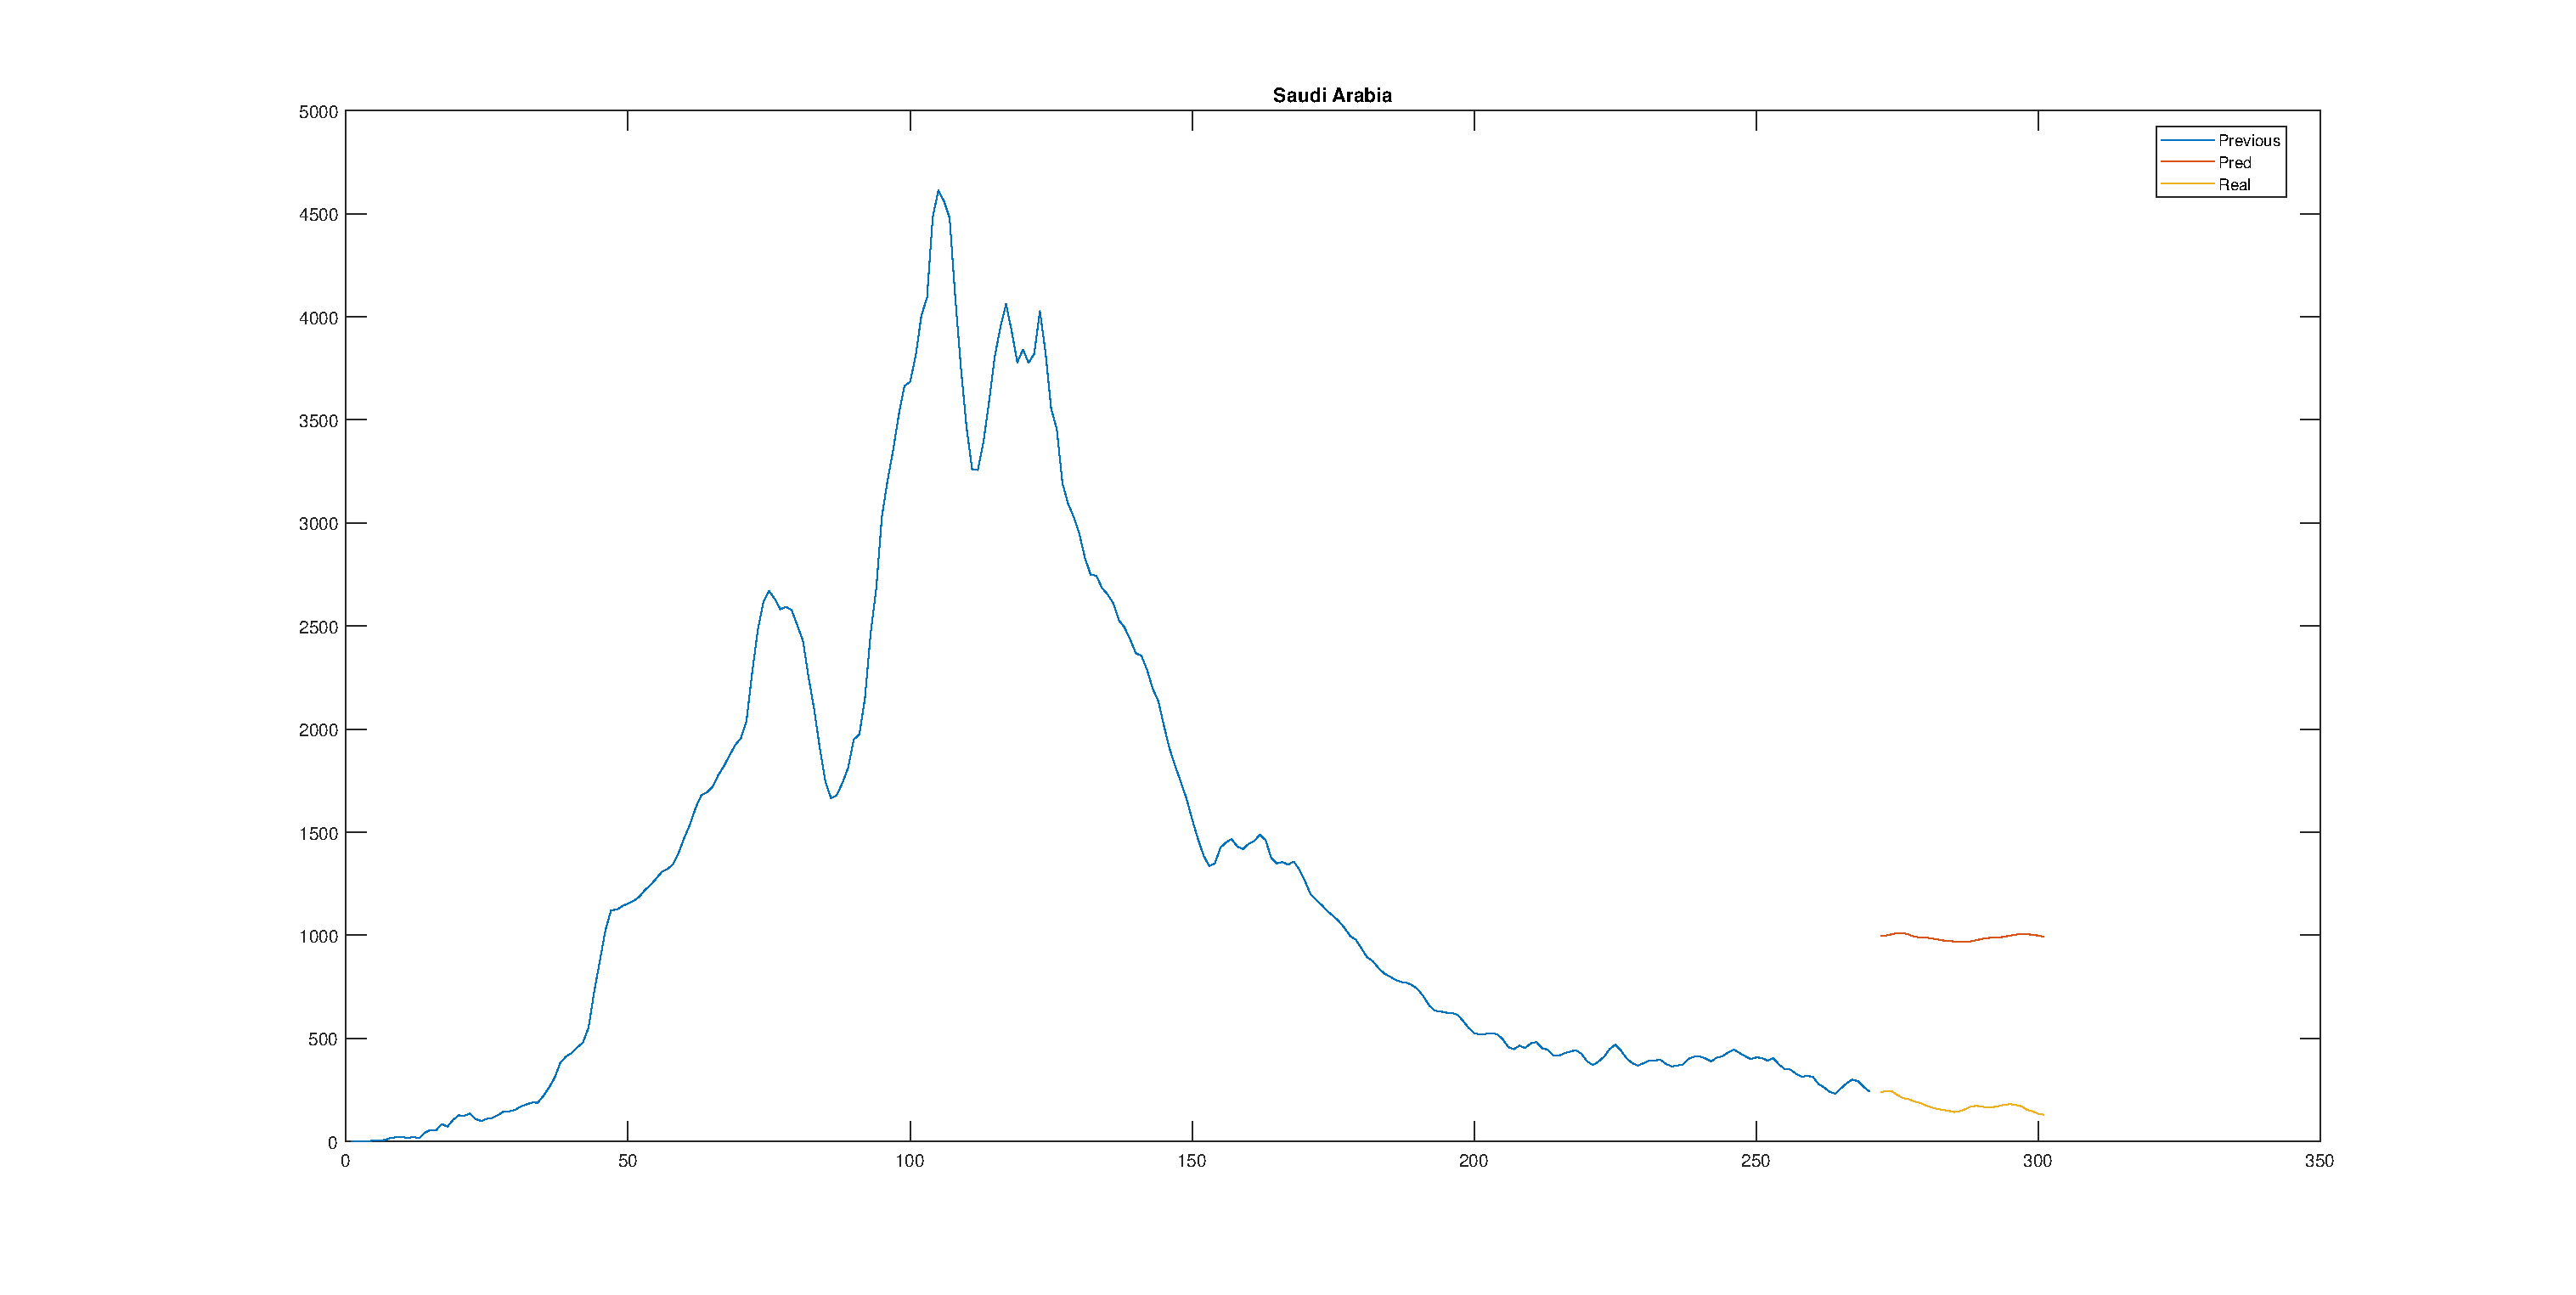
\includegraphics[height=8cm, width=10cm]{./Chap4/Pred4.eps}
            \vspace{-1.5em}
            \caption{对沙特阿拉伯的测试效果}
    \end{figure}
    \end{minipage}\\\quad\\
	  与简单模型一样,效果并不是很好. 这说明此种任务,在仅给到这些数据的情况下,对我们所构建的网络仍相当苦难. 想要达成我们上文所说的那种效果,只能提升数据处理,收集更多数据,抑或是进一步改变我们的网络的结构.

    \newpage
    \section{短期性分析第二种路径(基于时间序列特征的谱系聚类)}\label{第二种路径}
      本节相关的代码请详见\texttt{./Reports/Chapter6.mlx}.

      每日数据中的所有变量都是具有时间序列特征的,可以提取出来进行分析. 但是,每日数据中存在大量的数据缺失问题,在第\ref{数据的缺失值处理}节曾提到对于新增-累计数据的恢复问题,在这里就非常适用. 只是,当我们选取一个时段展开分析时,我们发现一些地区在某些字段上的数据全部缺失,以至于无从恢复,也不能通过插值方法拟合. 因此,我们不得不只选取一些数据完整的字段继续展开下面的分析.
    \subsection{构造特征}
      我们对$20$个地区在2021年10月1日至2022年1月1日的每日数据展开分析,由于一些地区的某些字段完全缺失,我们选取了\texttt{new\_cases},\texttt{total\_cases}和\texttt{stringency\_index}这三个字段,各自提取它们的时间序列特征,包括:
    \begin{itemize}
        \item 平均人口的峰峰值,即$(\max-\min)/\texttt{population}$;
        \item 平均人口的标准差,即$\texttt{std}/\texttt{population}$;
        \item 平均人口的平均值,即$\texttt{mean}/\texttt{population}$;
        \item 偏度\texttt{skewness};
        \item 峰度\texttt{kurtosis};
        \item 八日内的自相关系数之平均.
    \end{itemize}
    我们将所有获得的数据综合成一个$20\times (6\cdot 3)$的矩阵$\bm{X}$.
    \subsection{聚类分析}
      我们利用函数\texttt{pdist}, \texttt{squareform}, \texttt{linkage}和\texttt{dendrogram},对上面获得的数据$\bm{X}$谱系聚类.\\
    \begin{minipage}{\textwidth}
        \begin{figure}[H]
            \centering
            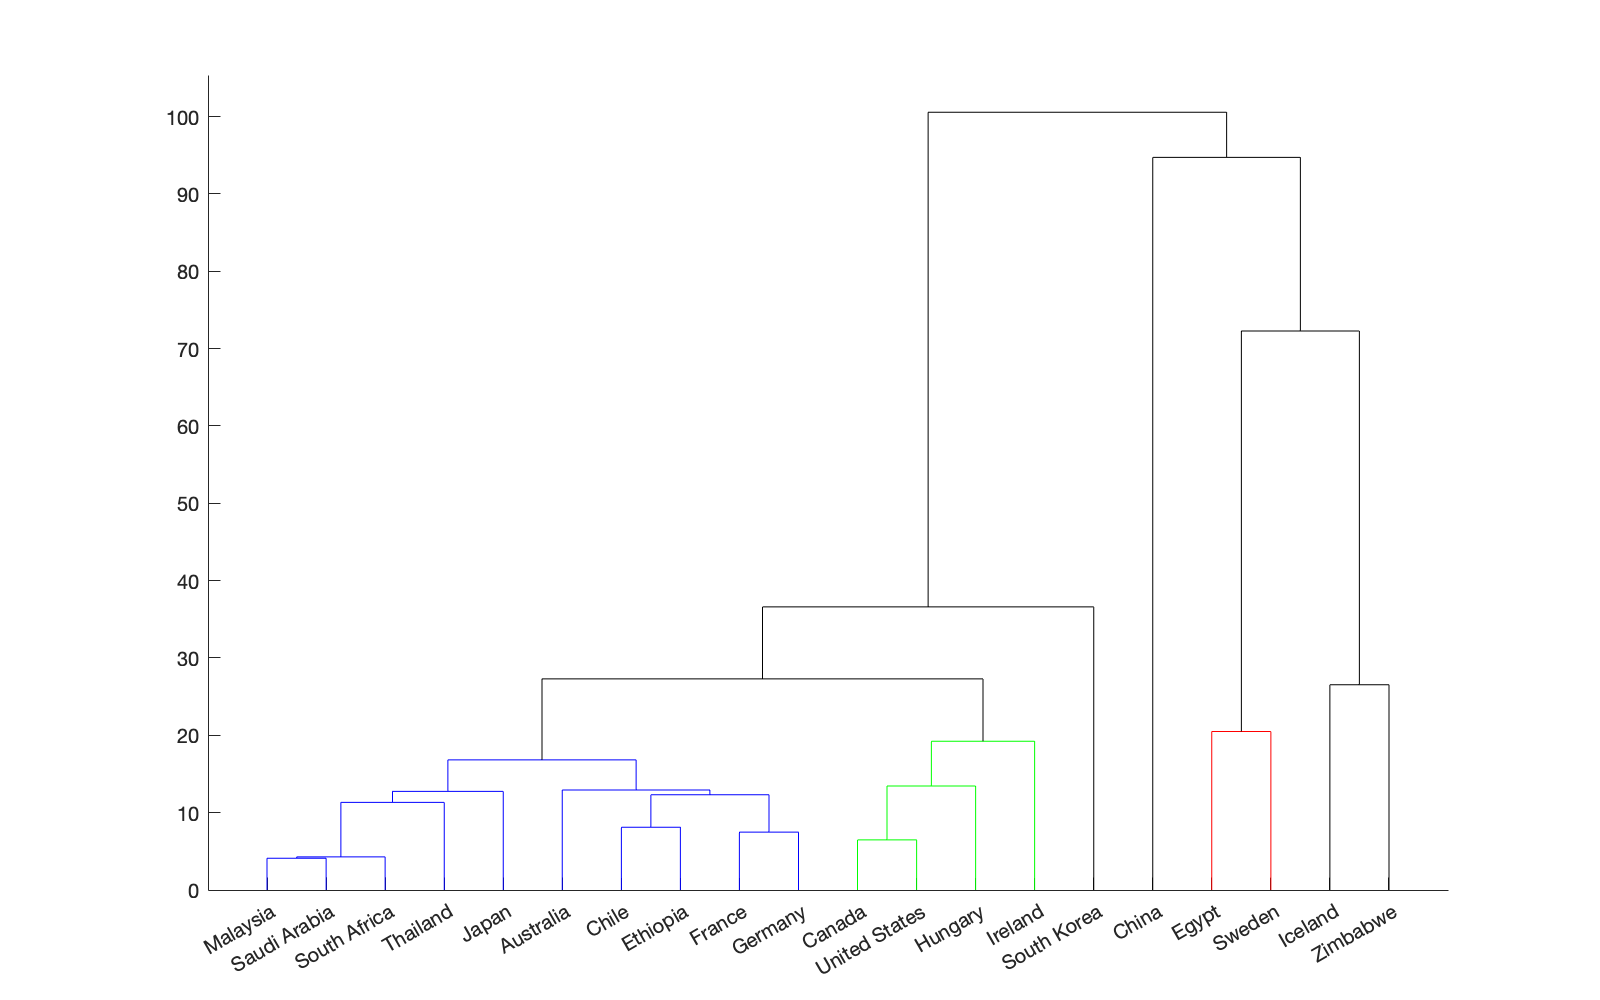
\includegraphics[width=0.9\textwidth]{./images/Tree_2.png}
            \vspace{-1em}
            \caption{基于时间序列的谱系聚类图}
            \label{images:Tree}
        \end{figure}
    \end{minipage}\\\quad\\
\begin{matlabcode}
Y = pdist(X);
Y = squareform(Y);
Z = linkage(Y);
dendrogram(Z, 'Labels', daily_location, 'ColorThreshold', 25);
\end{matlabcode}
      于是,对不同地区在疫情发展上的不同特征,我们就得到了一个具有树状结构的分类模型. 
    \subsection{小结}
    \begin{enumerate}
        \item [(1)] 对疫情发展的不同时期的数据提取时间序列特征,其结果往往是不同的,能反映出当下的疫情发展情况;
        \item [(2)] 在提取时间序列特征过程中,特征越多自然越能更全面地展现其发展状况,单一的特征往往不能揭示全部的信息;
        \item [(3)] 对各个地区的疫情发展情况进行谱系分析,首先能让我们对不同地区的情况有个大致的了解,知道哪些地区可能在面临着相似的问题与困境;其次,综合这些地区的情况,可以与其他的模型相结合,提出一些较为通用的政策建议.
    \end{enumerate}
    \newpage
    \section{其他的数据可视化与初步分析}\label{可视化}
      本节相关的代码请详见\texttt{./Reports/Chapter7.mlx}
    \subsection{Example 1: 每日新增病例与每日新增接种的综合分析}
        以法国的数据为例,利用\texttt{stackedplot}函数,作图如下:\\
        \begin{minipage}{\textwidth}
            \begin{figure}[H]
                \centering
                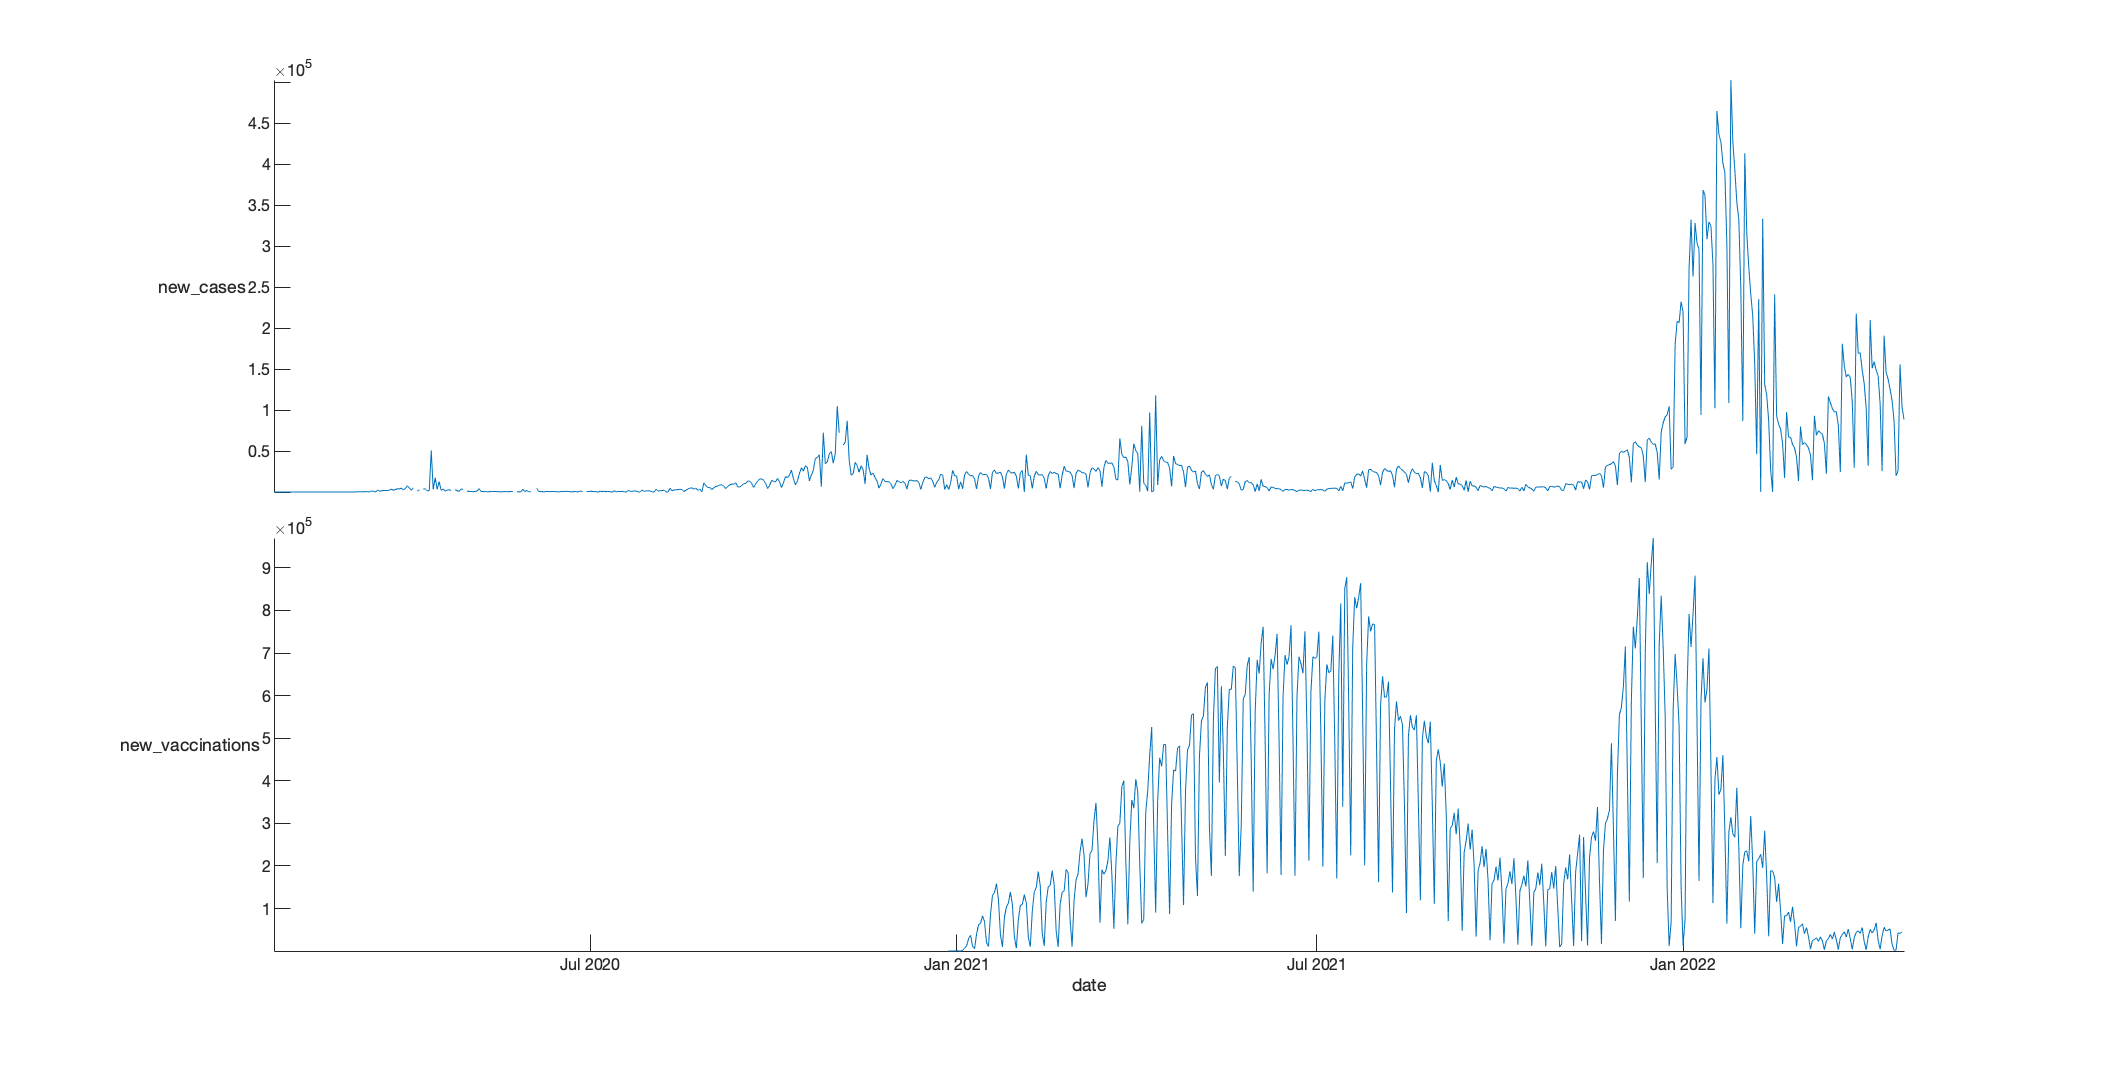
\includegraphics[width=0.9\textwidth]{./images/France_CasesAndVaccinations.png}
                \vspace{-1.5em}
                \caption{法国的每日新增病例与每日新增接种}
                \label{images:France_CasesAndVaccinations}
            \end{figure}
        \end{minipage}\\\quad\\
        我们知道,利用接种疫苗的方式,能在一定时间内降低易感人群感染的可能,但随着病原体不断变异,免疫逃逸现象随即产生,因此,新增接种数据与新增病例数据间可能存在的负相关性,也必定会随着时间的推进而趋于消失. 疫苗给人带来的免疫效果,究竟能延续多长时间,需要更多的数据进行分析. 这里,我们只是能从图中直接读出一定的负相关性.
        
    \subsection{Example 2: 缺失值处理前后累计病例数据的对比图像}
        仍以法国的数据为例. {\kaishu 本文行文中广泛选取法国数据为例的原因是,法国的数据有多次更正的情况,使得累计数据多个位点不单调,也使得对应日的新增数据缺失.}首先,作缺失值处理后图\ref{images:France_CasesAndVaccinations}的改变情况.\\
        \begin{minipage}{\textwidth}
            \begin{figure}[H]
                \centering
                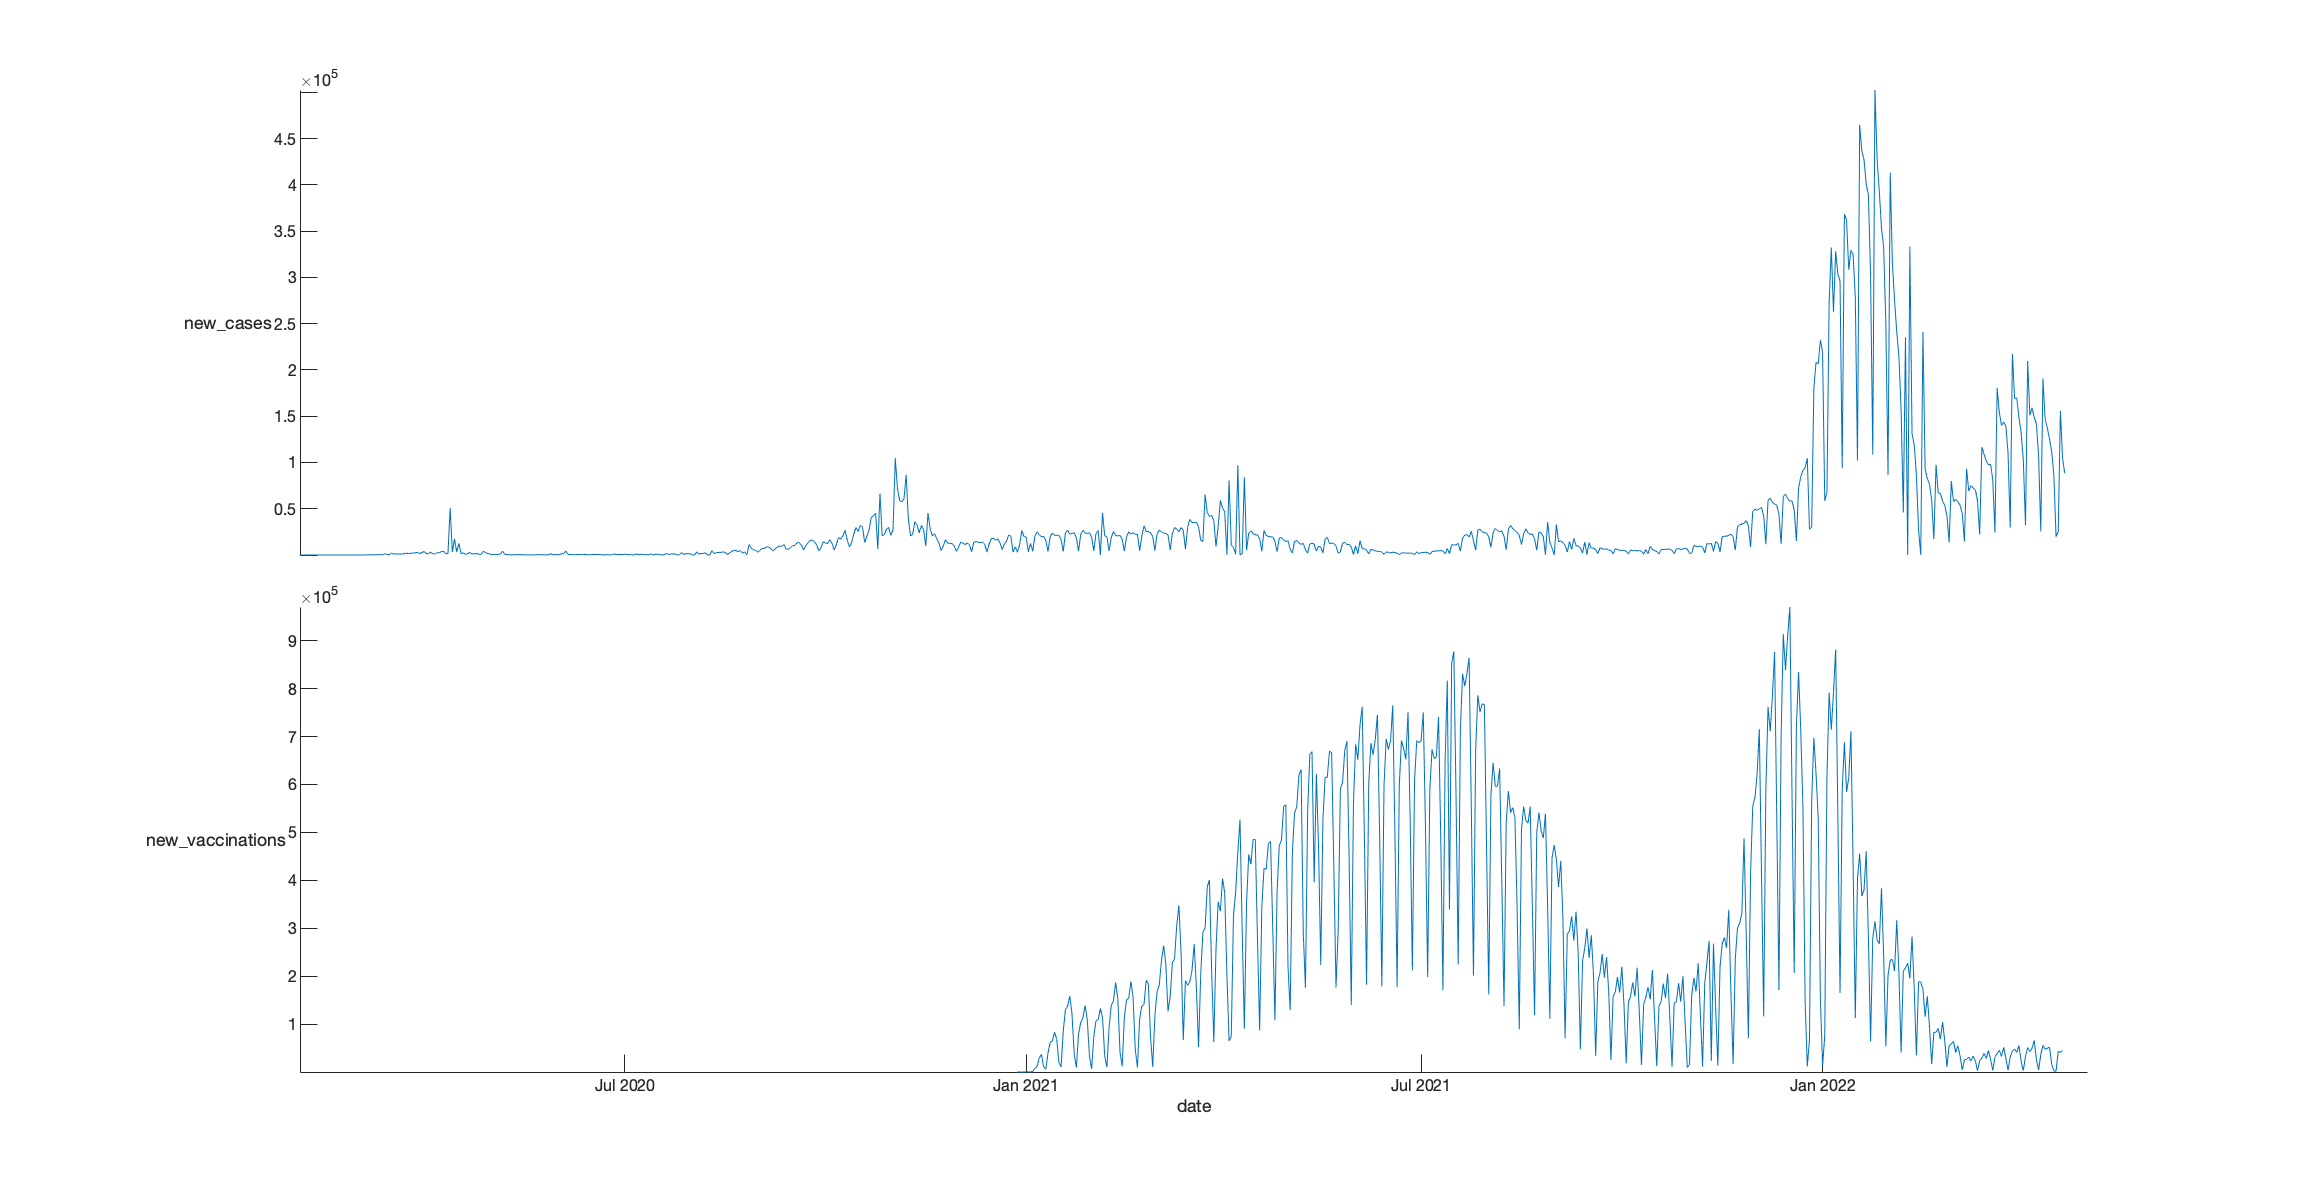
\includegraphics[width=0.9\textwidth]{./images/France_CasesAndVaccinations_2.png}
                \vspace{-1.5em}
                \caption{法国的每日新增病例与每日新增接种(缺失值处理)}
                \label{images:France_CasesAndVaccinations_2}
            \end{figure}
        \end{minipage}\\\quad\\
        可见疫情开始初期的一些断点已经相连. 然后对累计病例数据作图,上图是处理前的数据,下图是处理后的数据.\\
        \begin{minipage}{\textwidth}
            \begin{figure}[H]
                \centering
                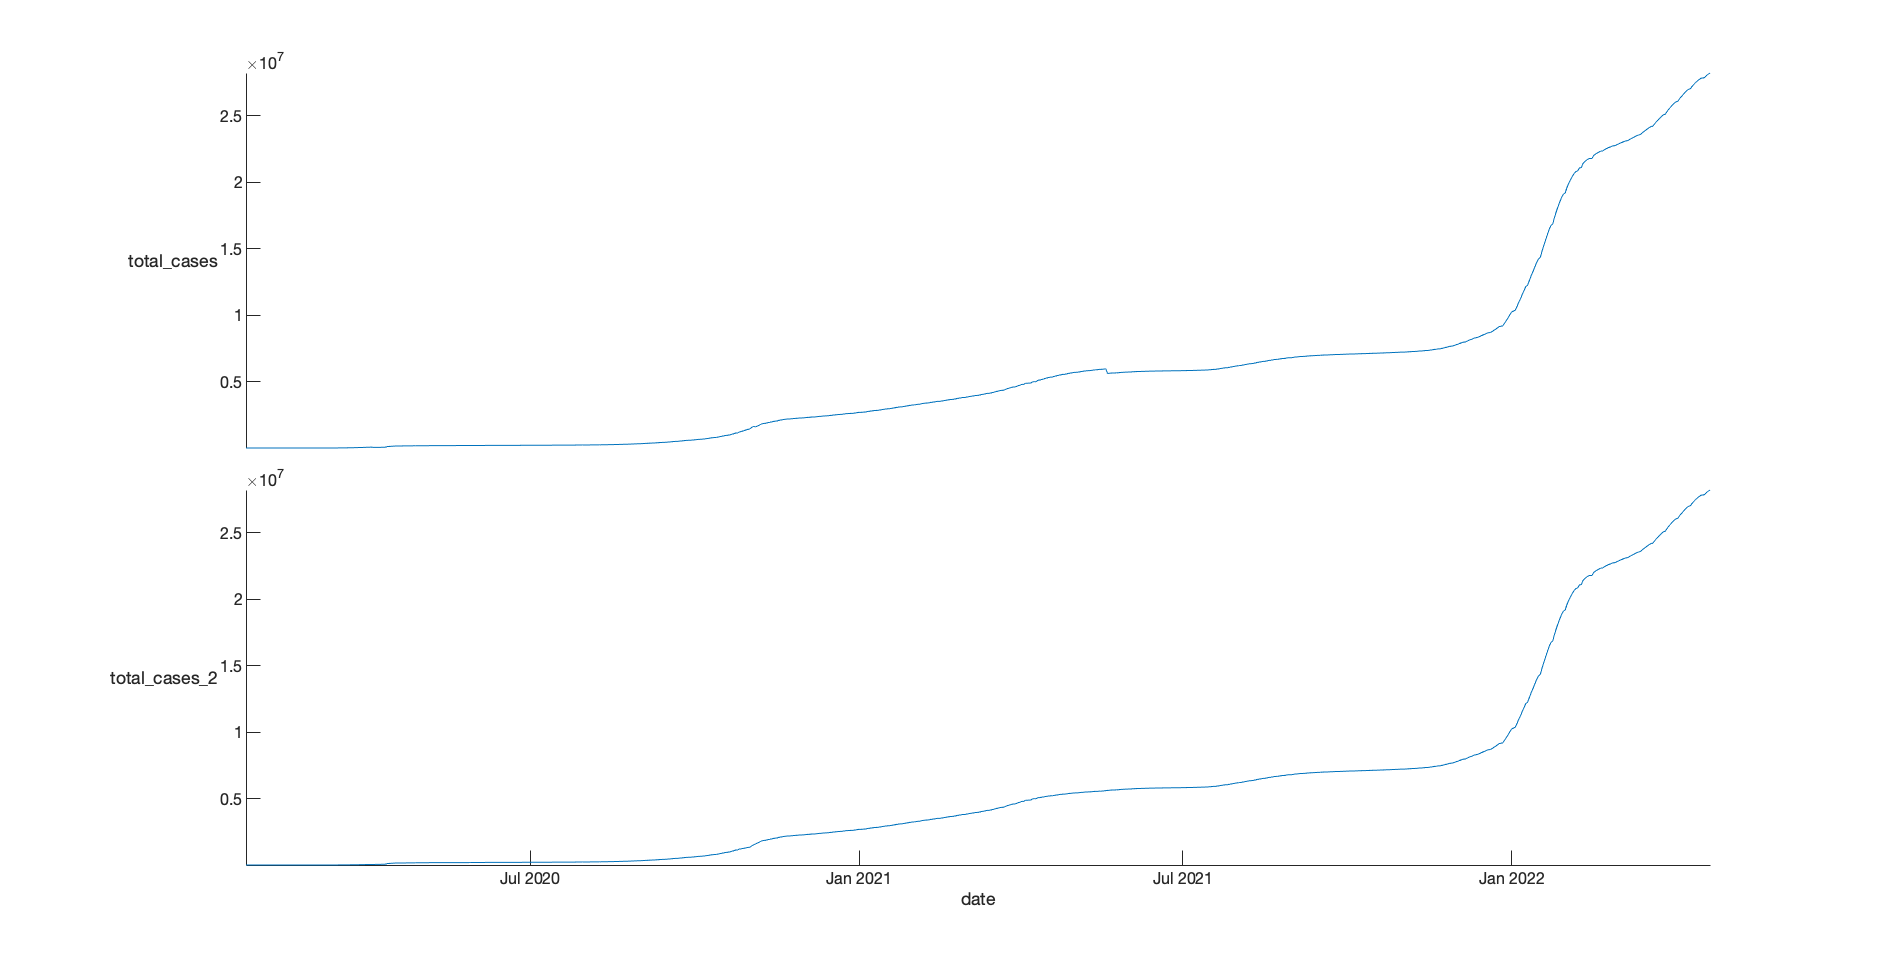
\includegraphics[width=0.88\textwidth]{./images/France_TotalCases.png}
                \vspace{-1.5em}
                \caption{法国的累计病例(缺失值处理)}
                \label{images:France_TotalCases}
            \end{figure}
        \end{minipage}\\\quad\\
        可见不单调的情况已被改善. 这里采用了节\ref{数据的缺失值处理}中提到的衰减分配. 根据不同的模型,可以选择不同的缺失值处理方式,这里不再赘述.
    \subsection{Example 3: ICU患者占全体住院患者的比例变化趋势}
    仍以法国的数据为例. \\
    \begin{minipage}{\textwidth}
        \begin{figure}[H]
            \centering
            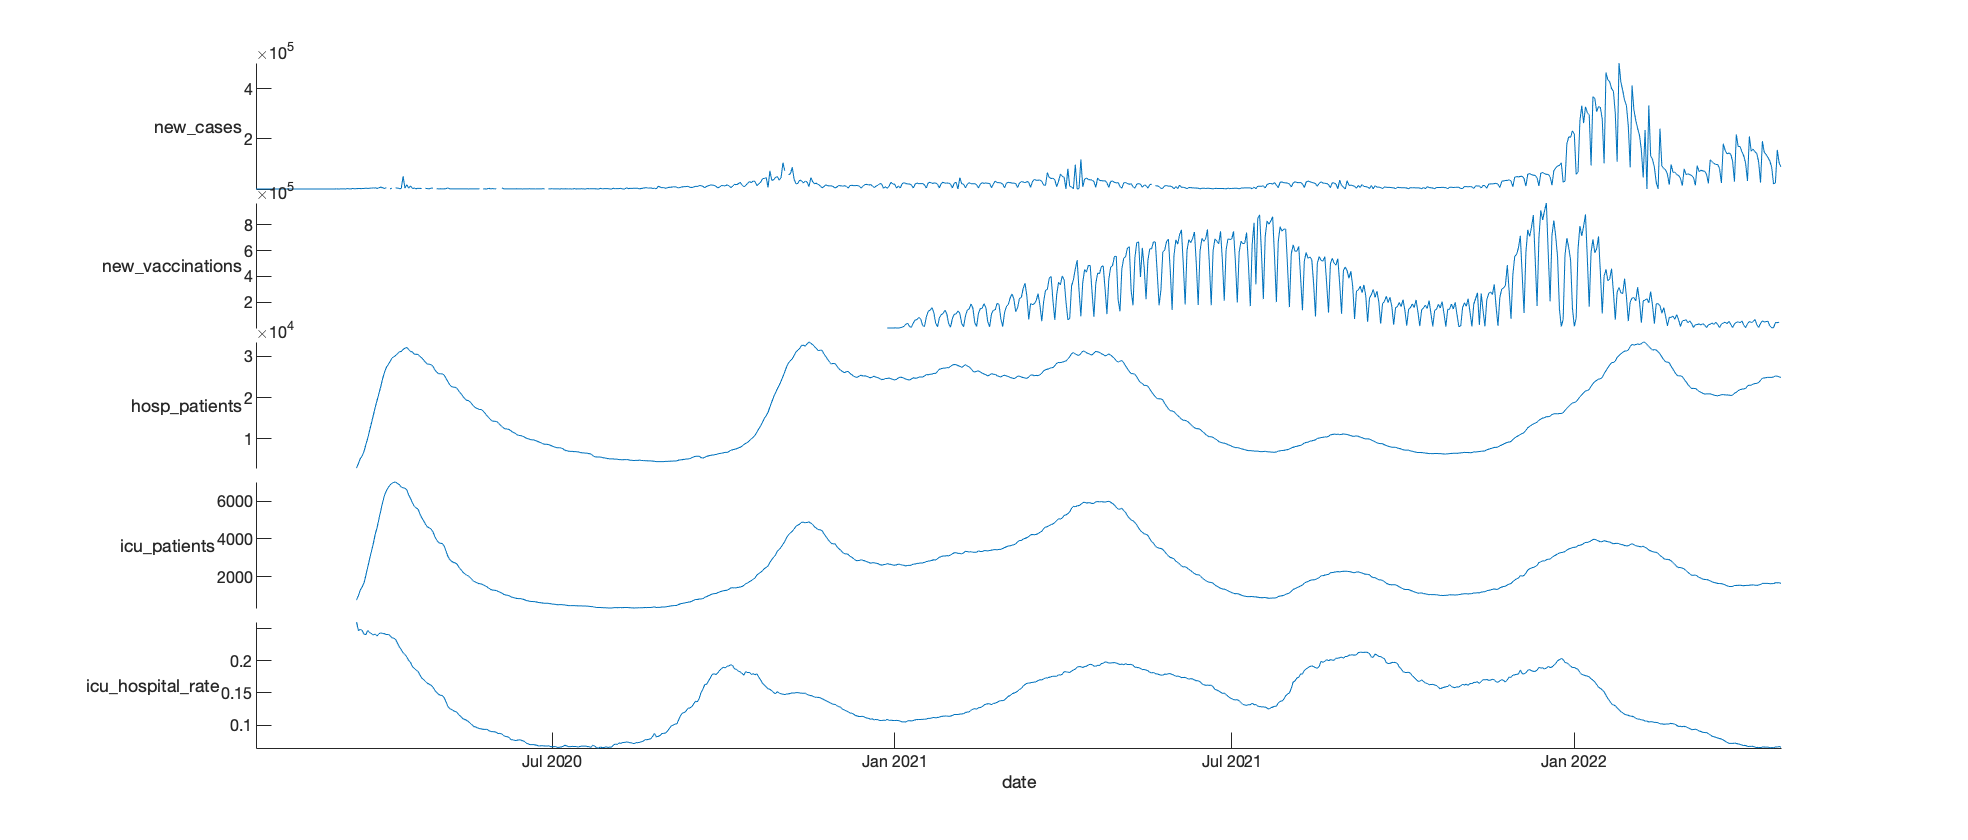
\includegraphics[width=\textwidth]{./images/France_ICU_Hospital.png}
            \vspace{-2em}
            \caption{法国的ICU患者占全体住院患者的比例变化趋势}
            \label{images:France_ICU_Hospital}
        \end{figure}
    \end{minipage}\\\quad\\
    住院患者数、重症监护患者数都是疫情严重程度的指标,而两者之比则可以反映优势病株的毒性. 图中可见,
    \begin{enumerate}
        \item [(1-)] 在先前多波疫情中,此三者的峰值点与新增病例数据的趋同;
        \item [(2-)] 在疫苗广泛接种之后的一段时期内,前两者的峰值均下降,但两者之比的峰值反而抬升({\kaishu 这意谓着这段时期内,一些轻症患者因为疫苗接种而避免了住院});
        \item [(3-)] 而在最近的疫情中,住院患者数跟随新增病例数据出现峰值,重症监护患者数小幅抬升,但两者之比近乎趋于$0$,可见优势病株的毒性正在减弱. 关于毒性减弱的度量,更进一步的分析需要更多的数据支持.
    \end{enumerate}
    \subsection{Example 4: 不同地区的检测阳性率(占比)变化趋势}
    阳性率(positive rate)是在特定地区的核酸检测中有多少份额确诊. 当一个地区的阳性测试率较低时,说明这些地区为防止疫情大规模爆发做出了很多努力;而当阳性率较高时,这通常意味着感染的真实数量可能远远高于确诊病例数.

      为了能对此项数据有更直观的认识,我们先对其进行了可视化:\\
    \begin{minipage}{\textwidth}
        \begin{figure}[H]
            \centering
            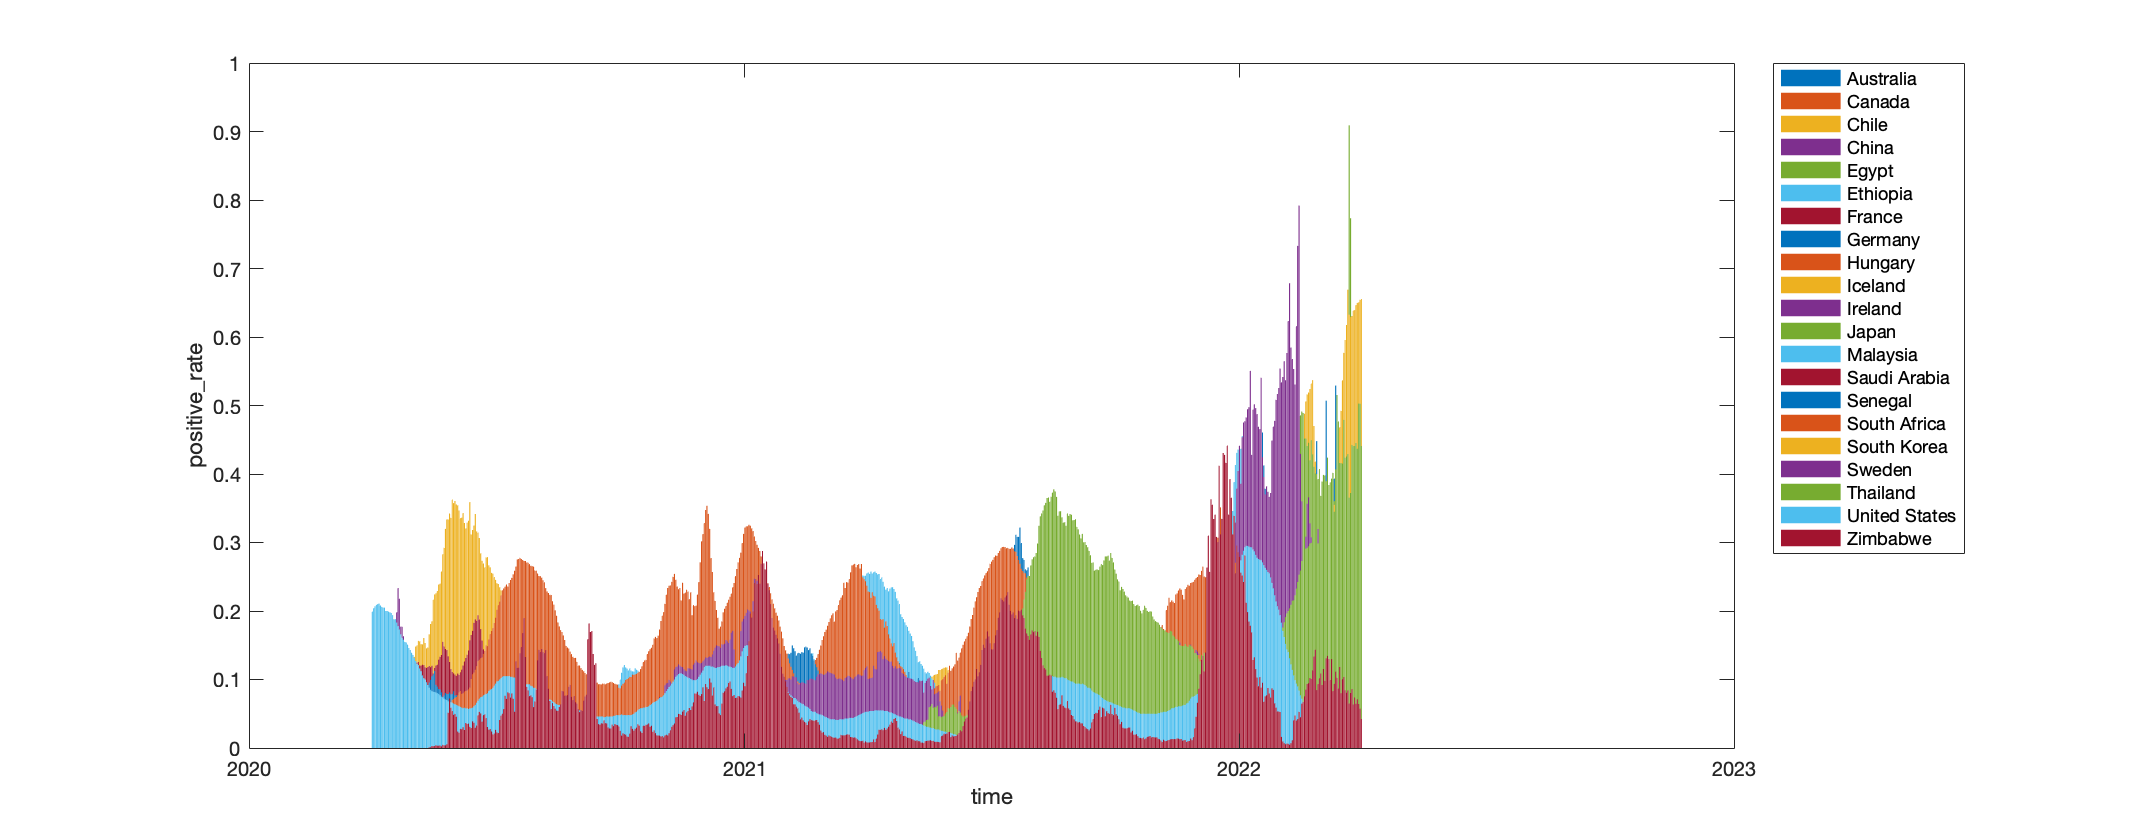
\includegraphics[width=1.1\textwidth]{./images/PositiveRate_1.png}
            \vspace{-2.5em}
            \caption{各国阳性率变化趋势}
            \label{images:PositiveRate_1}
        \end{figure}
    \end{minipage}\\\quad\\
    图中可以看到,阳性率变化呈现多个峰值,稍加对比可知这些峰值与新增病例数据的趋同,确能表征疫情的严重程度;且在最近一段时期,一些地区的阳性率大幅上升. 

      计算各国历时的最大阳性率,能够表征该国历时的疫情严重程度:\\
    \begin{minipage}{\textwidth}
        \begin{figure}[H]
            \centering
            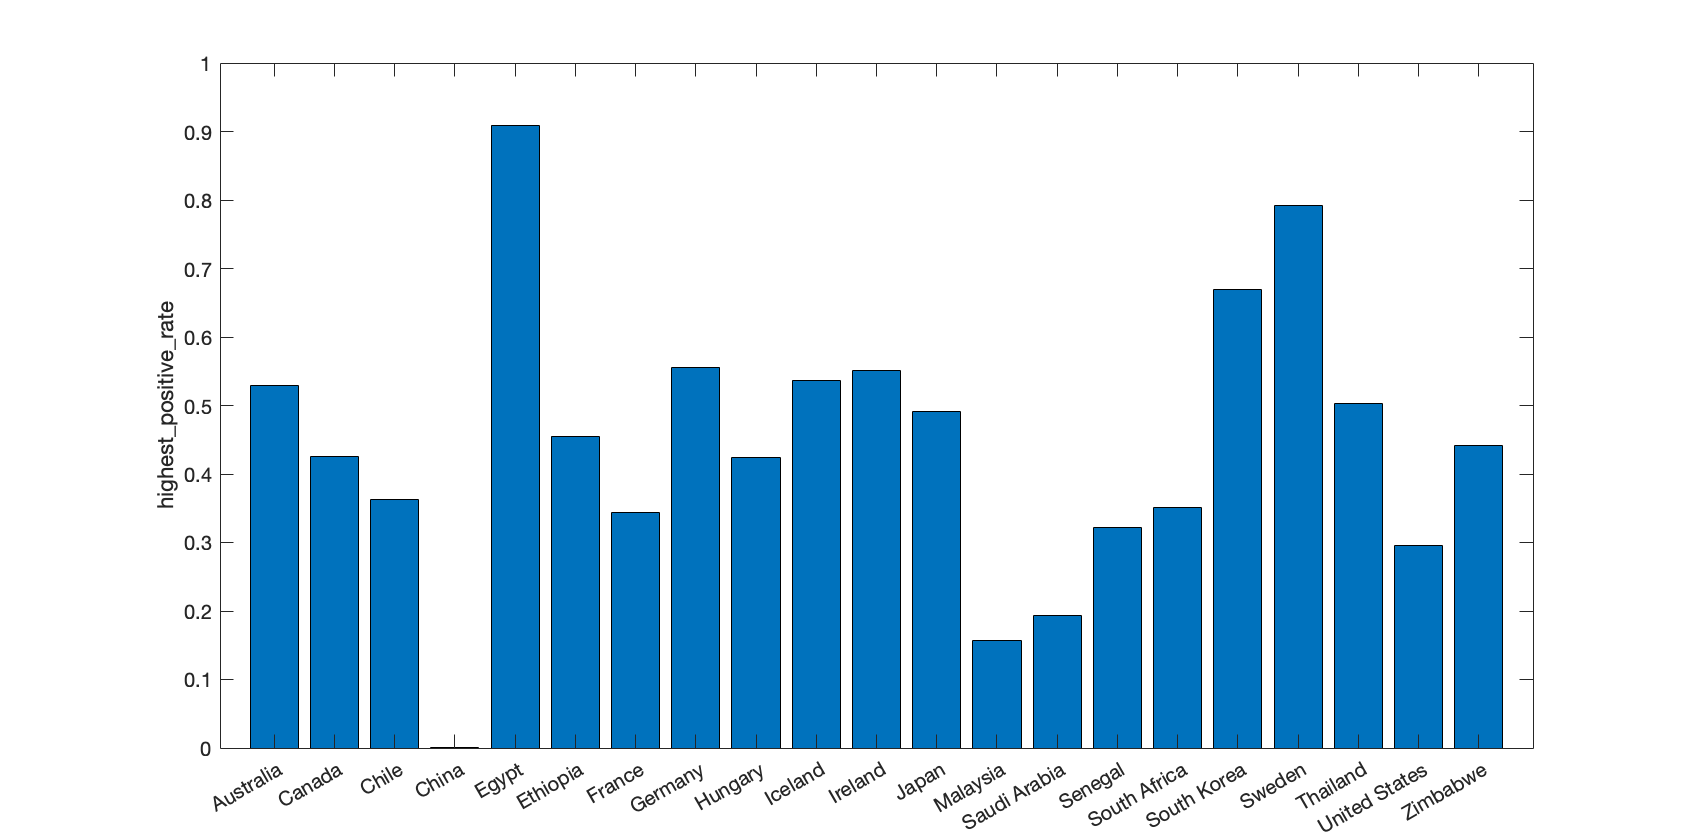
\includegraphics[width=\textwidth]{./images/PositiveRate_2.png}
            \caption{各国历时最大阳性率}
            \label{images:PositiveRate_2}
        \end{figure}
    \end{minipage}\\\quad\\
    由于加大检测量能够有效降低阳性率,因此不同地区的新增病例变化与阳性率变化情况有所不同,所以阳性率可以作为对不同地区疫情发展模式分类的一个不同于新增病例的指标. 

      按月分组取最大值作图如下,可以看出每个月份,在这$21$个地区中,疫情相对更严重的地区变化:\\
    \begin{minipage}{\textwidth}
        \begin{figure}[H]
            \centering
            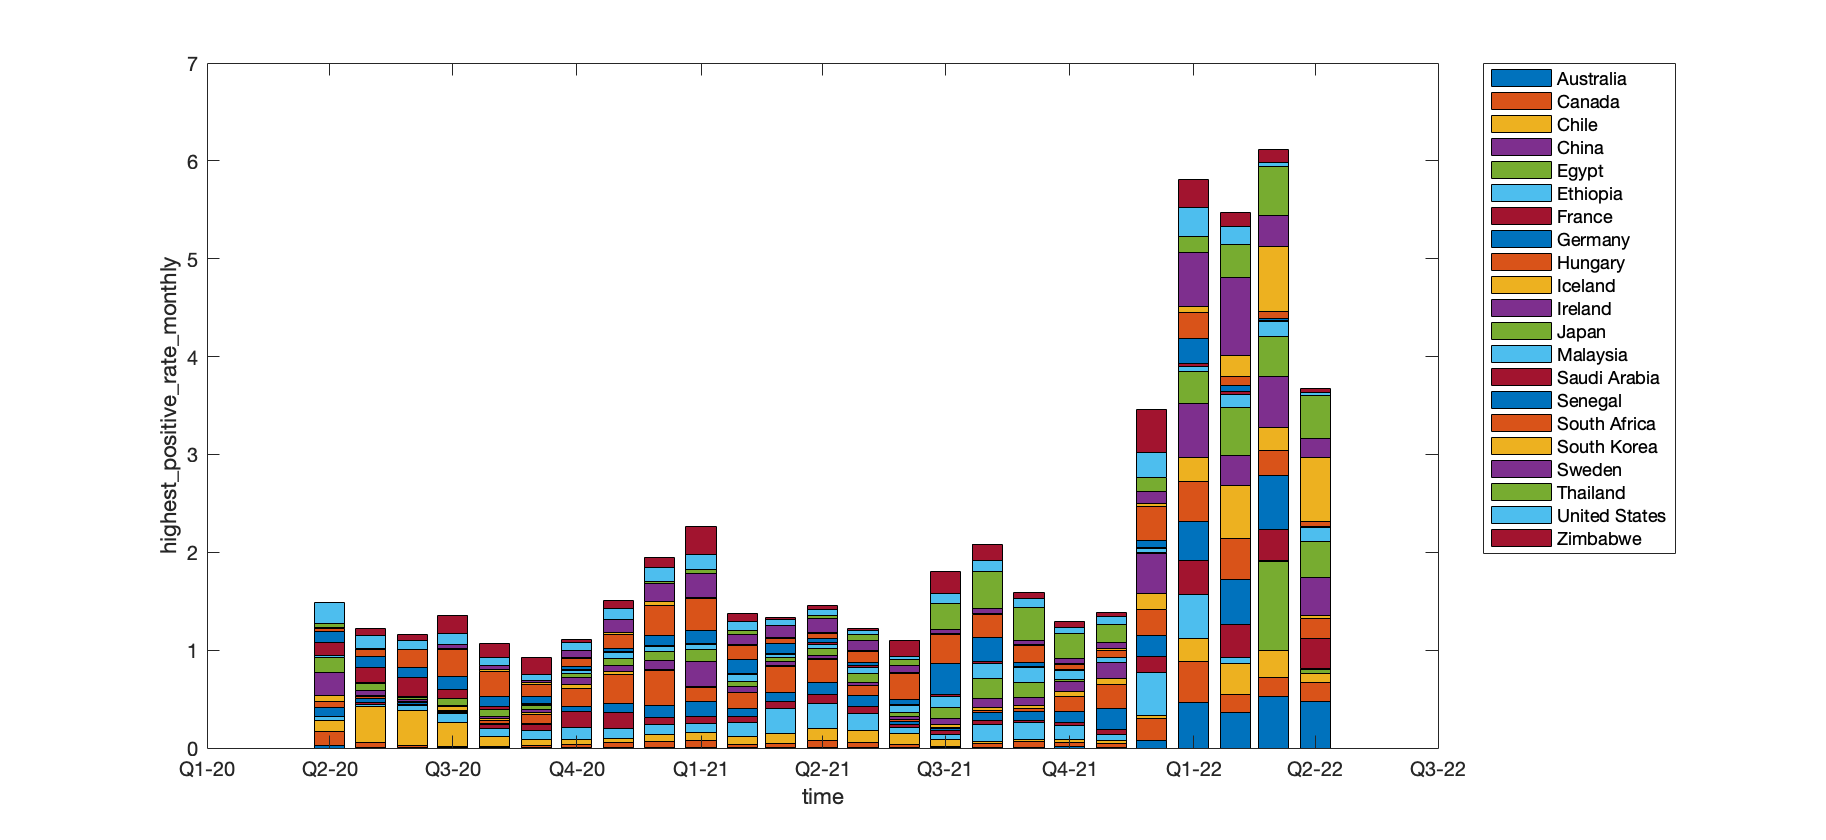
\includegraphics[width=\textwidth]{./images/PositiveRate_3.png}
            \vspace{-1.5em}
            \caption{各国阳性率变化趋势对比}
            \label{images:PositiveRate_3}
        \end{figure}
    \end{minipage}
    
    \vspace{5cm}
    \begin{center}
    以上就是我们对COVID-19数据集的分析,水平有限,多有疏漏,恳请各位指正. \\
    最后,感谢陈阳老师和两位助教一学期以来的指导与帮助!
    \end{center}
    \newpage
    \appendix
    \section{\texttt{StatisticsAnalysis}类}\label{app:StatisticsAnalysis}
      详见github仓库,网址\url{https://github.com/maix00/StatisticsAnalysis}. 本类存储在\texttt{./functions/@StatisticsAnalysis}. 本类目前有如下功能:
    \begin{enumerate}
        \item [1.] \textbf{修改导入参数,并导入表格};
        
        {\kaishu 
        修改导入参数,请使用\texttt{ImportOptions}参数,类型可以是\texttt{struct}或采用name/value-pair的\texttt{cell};name应当是你所要修改的\texttt{detectImportOptions}中得到的属性. 
        
          另外,如果有设置多个导入参数的需要,请将值置于\texttt{1x1 cell},比如导入第$3\sim 10$及$20\sim 30$行,则为\texttt{DataLines:\{\{[3 10] [20 30]\}\}}.
        }
        \item [2.] \textbf{检索表格};
        
        {\kaishu
        传入检索参数,请使用\texttt{SelectTableOptions},类型可以是\texttt{struct}或采用name/value-pair的\texttt{cell};name应当是你所要检索的变量名.

          导入与检索后的表格,可以通过属性名\texttt{Table}或\texttt{TimeTable}访问. 访问原表格请使用属性名\texttt{WholeTable}. 
        }
        \item [3.] \textbf{缺失值探测、修正};
        
        {\kaishu
        传入修正缺失值的参数,请使用\texttt{MissingValuesOptions},类型可以是\texttt{struct}或\texttt{N\_} \texttt{by\_3 cell}. 传入\texttt{cell}时,每行第一位是涉及的变量名\texttt{VariableNames},第二位是使用的修正方法\texttt{Style},第三位是该修正方法所需要的其他参数,类型可以是\texttt{struct}或者采用name/value-pair的\texttt{cell}.

          查看探测信息,请使用属性名\texttt{MissingValuesReport}. 缺失值修正后的表格将覆盖掉\texttt{obj.Table}. 此外,允许的参数值如下表所示:
        \vspace{-2em}
        \begin{flushleft}
        \begin{tabular*}{\textwidth}[H]{c|l|l}
            修正方法&参数名&允许参数值\\ \hline
            \texttt{MissingDetect}&——&——\\ \hline
            \multirow{11}{*}{
                \makecell{\\
                \texttt{Increment-}\\\texttt{Addition}
                }
            }
            &\texttt{RemoveLastRows}
            &缺省\texttt{true}\\ \cline{2-3}
            &\texttt{ConstantValues\_FirstRows}
            &缺省空\\
            &\texttt{RemoveFirstRows}
            &缺省\texttt{true}\\ \cline{2-3}
            &\texttt{InterpolationStyle}
            &\multirow{6}{*}{
                \makecell{
                \texttt{Style}缺省\texttt{"Linear"}或\\\texttt{"LinearRound"},
                允许函数名\\字符串如\texttt{"spline"};\\\texttt{Function}允许函数句柄.
                }
            }\\
            &\texttt{InterpolationFunction}
            &\\
            &\texttt{InterpolationStyle\_P}
            &\\
            &\texttt{InterpolationFunction\_P}
            &\\
            &\texttt{InterpolationStyle\_C}
            &\\
            &\texttt{InterpolationFunction\_C}
            &\\ \cline{2-3}
            &\texttt{DecreasingAdditionStyle}
            &\multirow{2}{*}{
                \makecell{\texttt{Style}缺省\texttt{"Exponential"},允许\\\texttt{"LinearScale"}, \texttt{"DoNothing"}.}
            }\\
            &\texttt{DecreasingAdditionParameters}
            &\\
            \hline
            \multirow{2}{*}{
                \makecell{
                \texttt{Interpolation}
                }
            }
            &\texttt{InterpolationStyle}
            &\\
            &\texttt{InterpolationFunction}
            &\\\hline
            \texttt{ConstantValues}
            &\texttt{ConstantValues}
            &缺省空
        \end{tabular*}
        \end{flushleft}

        其中,函数句柄句法、相关参数有
        \begin{enumerate}
            \item [(1-)]\texttt{T = InterpolationFunction(T, startRow, endRow, VariableMap);}
            \item [(2-)]\texttt{T = InterpolationFunction\_C(T, startRow, endRow, IncrementWhere, Ad-}\\\texttt{ditionWhere);} 注:新增-累计类数据会有两种需要插值的情况,记为$P$与$C$.
            \item [(3-)] 非单调累计数据处理方法\texttt{"Exponential"}的参数较多,包括RoundingWindowAhead, RoundingWindowBehind, RoundingStrategy, RoundingScale, ExponentialRate, AcceptedRatioMinimum, AcceptedRatioMaximum, SpanAheadSkip.
        \end{enumerate}

        注:缺失值处理的功能还在测试阶段,不可避免还有些问题,欢迎批评指正!
        }
        
        \item [4.] \textbf{给不同变量贴上不同标签,并对不同标签的变量,计算传入或预设的统计指标,并将计算结果添加到\texttt{Table.Properties.CustomProperties}}.
        
        {\kaishu
        传入标签与统计指标的参数,请使用\texttt{TagsGenerateOptions},类型可以是\texttt{struct}或\texttt{cell};\texttt{struct}的域名,或者\texttt{cell}的左列,应当是函数\texttt{./function/@StatisticsAna-} \texttt{lysis/TagsGenerate}的参数名,包括
        \begin{itemize}[itemsep=-1pt,topsep=1pt]
            \item \texttt{CustomTagName},例如\texttt{\{"continuous", [0 1 1]\}};
            \item \texttt{CustomTagFunction},例如\texttt{\{"continuous", "variance", @(x,y)tsnanvar(x)\}},其中\texttt{x}和\texttt{y}分别是变量所在列全体,及其去重无缺全体.
        \end{itemize} 
        }
    \end{enumerate}

    注:
    \begin{enumerate}
        \item [(1)] 检索功能引用了\texttt{./function/selecttable.m}与MATLAB内置类\texttt{timerange}.
        \item [(2)] 缺失值修正引用了\texttt{./function/@TableMissingValues}.
        \item [(3)] 更新各种参数可以使用类方法\texttt{Update}.
        \item [(4)] 新增-累计类数据的两种需要插值的情况,记为$P$与$C$,指的是缺失值在尽可能通过加减恢复之后,其所在位置连成一片后的形状,分别如下图左右所示. 其中$I$表示增量数据,$A$表示总量数据,方框表示缺失值. 在这两种情况下,不能仅凭简单的加减恢复数据,必须通过插值.
    
    \begin{minipage}{\textwidth}
    \centering
    \begin{tikzpicture}[scale=0.8]
        \draw (0,0) -- (1,0) -- (1,3) -- (0,3) -- (0,0);
        \draw (0,1) -- (2,1) -- (2,3) -- (1,3);
        \draw (0,2) -- (2,2);
        \coordinate [label=90:$I$] (I) at (0.5,3);
        \coordinate [label=90:$A$] (A) at (1.5,3);
        \coordinate [label=-90:$(P)$] (P) at (1,-3);
    \end{tikzpicture}
    \quad\quad
    \begin{tikzpicture}[scale=0.8]
        \draw (0,0) -- (1,0) -- (1,3) -- (0,3) -- (0,1) -- (2,1) -- (2,3) -- (1,3);
        \draw (0,2) -- (2,2) -- (2,0) -- (1,0) -- (1,-1) -- (0,-1) -- (0,0);
        \coordinate [label=90:$1$] (P1) at (0.5,0.2);
        \coordinate [label=90:$I$] (I) at (0.5,3);
        \coordinate [label=90:$A$] (A) at (1.5,3);
        \coordinate [label=-90:$(C1)$] (C1) at (1,-3);
    \end{tikzpicture}
    \quad\quad
    \begin{tikzpicture}[scale=0.8]
        \draw (0,0) -- (1,0) -- (1,3) -- (0,3) -- (0,1) -- (2,1) -- (2,3) -- (1,3);
        \draw (0,2) -- (2,2) -- (2,0) -- (1,0) -- (1,-1) -- (0,-1) -- (0,0);
        \draw (2,0) -- (2,-1) -- (1,-1) -- (1,-2) -- (2,-2) -- (2,-1);
        \draw (1,-2) -- (0,-2) -- (0,-3) -- (1,-3) -- (1,-2);
        \coordinate [label=90:$1$] (P1) at (0.5,0.2);
        \coordinate [label=90:$2$] (P2) at (0.5,-1.8);
        \coordinate [label=90:$I$] (I) at (0.5,3);
        \coordinate [label=90:$A$] (A) at (1.5,3);
        \coordinate [label=-90:$(C2)$] (C2) at (1,-3);
        \coordinate [label=0:$\cdots\cdots$] (CD) at (2.5,0.25);
    \end{tikzpicture}
    \end{minipage}\\\quad\\
    代码实现的过程,简单来说,就是识别出这两种缺失形状,再分别插值的过程. 这样之后,再额外考虑总量数据不单调的问题. 针对这个插值的功能,为了演示,我们提供了一些极端的个例,请参见文件\texttt{./functions/@TableMissingValues/Example\_TableMissingValues.mlx}.

    \newpage
    \section{本文所使用的MATLAB代码存储结构}\label{存储结构}
    以本文所在文件夹为当前文件夹. 
    \begin{itemize}
        \item \texttt{./Project.prj}文件是MATLAB自带的文件类型,双击点开可以用来添加路径. \texttt{./resources}文件夹是MATLAB上述功能的载体.
        \item \texttt{./functions}文件夹包含一些作为基础设施的类与函数,主要包括
            \begin{itemize}
                \item \texttt{./functions/@StatisticsAnalysis}类. 用于导入、检索、分析表格.
                \item \texttt{./functiions/@TableMissingValues}类. 用于探测与处理表格缺失值.
                \item \texttt{./functions/selecttable.m}函数. 用于检索表格.
            \end{itemize}
        \item \texttt{./Reports}文件夹包括本文全部行文所需的代码,包括以下的文件:
            \begin{itemize}
                \item \texttt{./Reports/Chapter3.mlx}. 关于缺失值处理.
                \item \texttt{./Reports/Chapter4.mlx}. 关于自回归分析.
                \item \texttt{./Reports/Chapter5.mlx}. 关于$k$-mean聚类与LSTM神经网络模型. 其功能函数存储在\texttt{./src}文件夹中.
                \item \texttt{./Reports/Chapter6.mlx}.
                \item \texttt{./Reports/Chapter7.mlx}. 关于其他的数据可视化与初步分析.
            \end{itemize}
        \item 其他一些文件具有辅助作用,例如画图等,这里不做展开.
    \end{itemize}
\end{enumerate}
\end{document}


